\documentclass[twocolumn,10pt]{article}

\usepackage{graphicx}
\usepackage{amsmath}
\usepackage{natbib}
\usepackage{geometry}
\usepackage{hyperref}
\usepackage{booktabs}

\geometry{margin=0.75in}

\title{LITTORAL: A Geometric Analysis of Global Relative Sea-Level Indicators Under Rotational Reorganization Hypotheses}
\author{Craig Stone}
\date{\today}

\begin{document}

\maketitle

\begin{abstract}
We present a global, geocoded compilation of relative sea-level (RSL) indicators---including submerged and raised beaches, reef terraces, sedimentary markers, and geomorphic shoreline features---assembled into the LITTORAL dataset. Spanning a vertical range of approximately $\pm 200$~m relative to present sea level, this dataset enables a geometry-first interrogation of global sea-level structure independent of conventional forward models. 

We compute the first-order spatial gradient of the LITTORAL elevation field and compare its structure to a pre-existing anisotropy field (the Mach field) derived from digital elevation model (DEM) flow alignment. The comparison reveals a non-random correspondence: preferred gradient pathways align with low-penalty Mach corridors, while high-penalty regions are systematically avoided. 

Conditioned discrimination tests, comparing observed candidate axes to matched random ensembles, demonstrate statistically significant reductions in integrated path penalties. These results support the hypothesis that global RSL indicators encode a coherent geometric structure consistent with large-scale redistribution processes. 

We further introduce a geodetic inverse test in which reported shoreline elevations are mapped into candidate polar-offset orientations. Using the Beebe (1931) Bermuda submerged-beach report as a descriptive anchor, we show that low-amplitude shoreline indicators and extreme-depth anomalies occupy different regions of the inverse solution space. This motivates a depth-regime interpretation in which shallow, deep, and raised indicators are treated not as a single homogeneous population, but as potentially distinct geometric regimes.

We interpret this structure in the context of geodetic sea-level change as described by \citet{fairbridge1961}, and explore its implications for rotational reorganization frameworks.
\end{abstract}

\section{Plain Language Summary}

Sea level is often treated as a simple global rise or fall. But the geological record tells a more complex story. Around the world, we find beaches, reefs, and shoreline features at many different heights---some far above today's oceans, others deeply submerged. 

In this study, we bring together thousands of these observations into a single global dataset and ask a different question: \emph{what shape do these data form?} Instead of assuming a cause, we examine the geometry directly.

We find that these sea-level markers are not randomly distributed. Instead, they follow preferred pathways across the Earth’s surface, forming a pattern that aligns with an independently derived global anisotropy field. This suggests that past sea-level changes may have been influenced by large-scale redistributions of mass or rotation, rather than purely local or gradual processes.

A useful example is William Beebe’s 1931 report of beach-like material dredged from more than 2.5 km below present sea level south of Bermuda. Beebe described water-worn pebbles, coral fragments, and shallow-water shells at abyssal depth. In this paper we use that observation not as proof of a mechanism, but as a clear descriptive anchor: if a former beach is now very deep, what kind of geodetic rotation geometry would be required to make such an elevation possible?

\section{Introduction}

The interpretation of relative sea-level (RSL) indicators has traditionally proceeded through forward models of eustatic change, glacio-isostatic adjustment (GIA), and tectonic uplift or subsidence. While these frameworks have achieved considerable explanatory power, they inherently impose causal structure prior to analysis.

An alternative approach is to treat the global distribution of RSL indicators as a geometric field and to interrogate its structure directly. This perspective aligns with the classical observations of \citet{fairbridge1961}, who emphasized that geodetic sea-level change may arise from redistribution of the Earth's mass and rotational geometry, rather than purely volumetric ocean change.

Fairbridge noted that:
\begin{quote}
Sea-level change is not simply a matter of adding or subtracting water, but involves the deformation of the geoid and the redistribution of the oceanic bulge under changing rotational conditions.
\end{quote}

This study revisits that perspective using modern data and computational tools. We assemble a global dataset of RSL indicators (LITTORAL) and examine its spatial structure through gradient analysis and comparison with an independently derived anisotropy field (the Mach field). The Mach compatibility field, defined as a constraint-based measure of Euler flow admissibility over the Earth's surface \citep{stone2026_euler_mach}, provides an independent anisotropy structure against which the LITTORAL gradient may be evaluated.

\section{Data: The LITTORAL Dataset}

The LITTORAL dataset comprises 3176 geocoded observations of relative sea-level indicators, compiled from published literature and databases including WALIS. Each record includes:

\begin{itemize}
\item Geographic coordinates (latitude, longitude)
\item Elevation or depth relative to present sea level
\item Indicator type (e.g., beach, reef, sedimentary marker)
\item Source reference
\end{itemize}

The dataset spans a vertical range of approximately $-200$~m to $+200$~m and provides global coverage across continental margins and ocean basins.

\begin{figure}[ht]
\centering
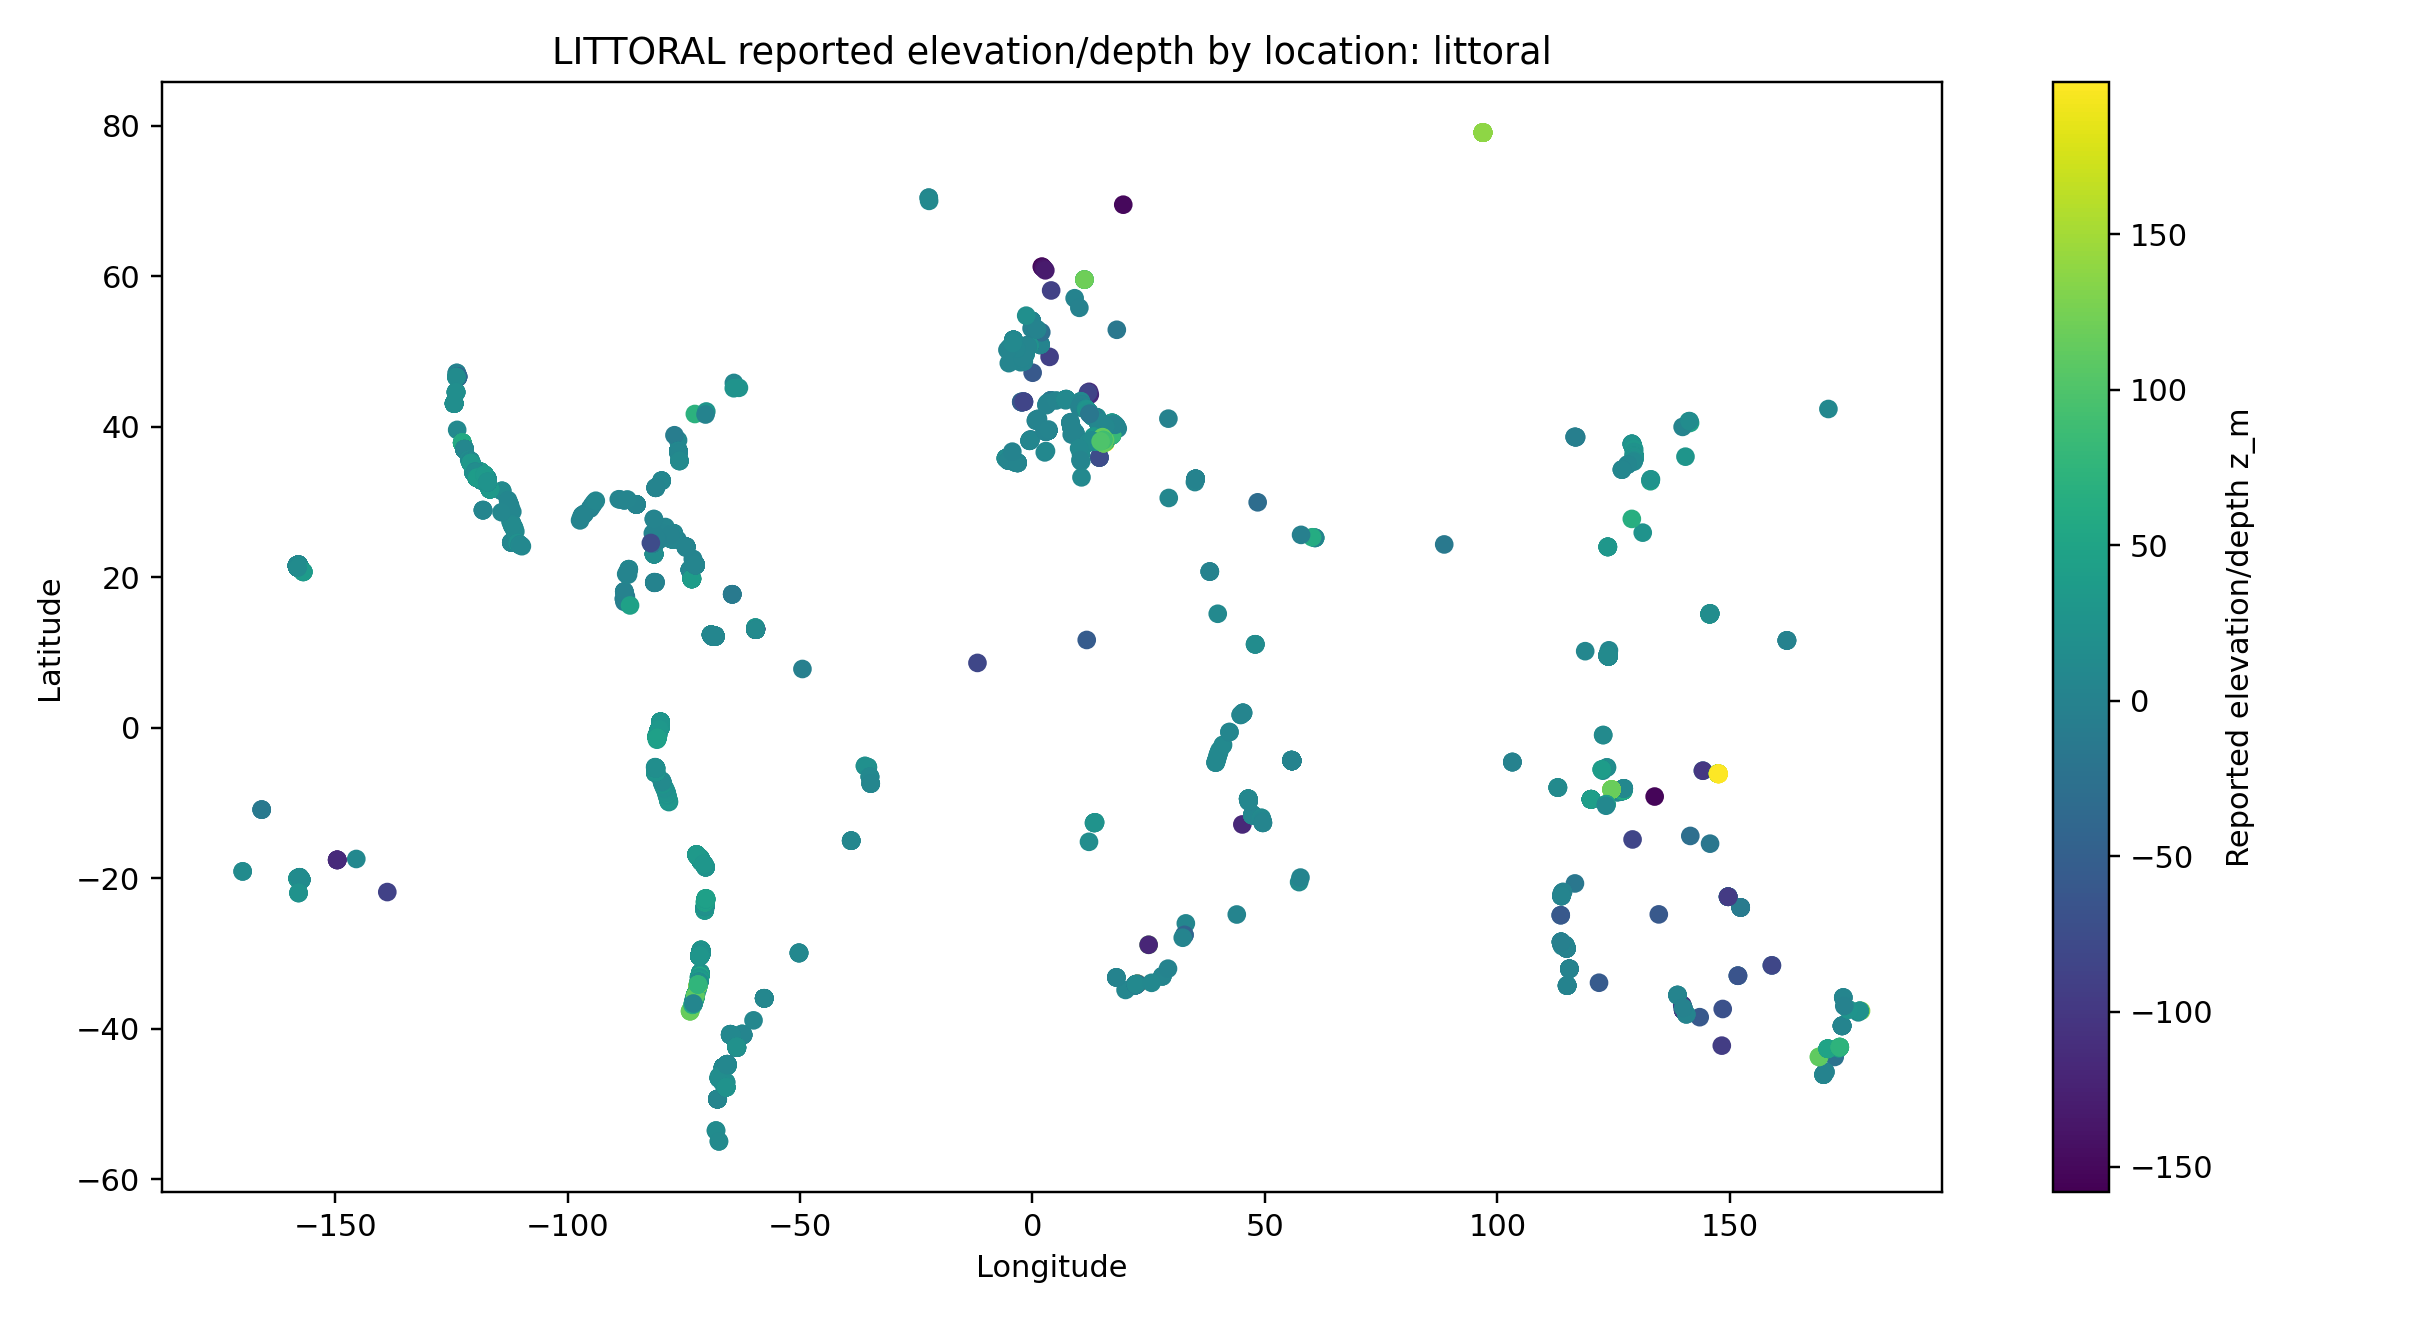
\includegraphics[width=\columnwidth]{../outputs/geospatial_01/01_littoral_global_scatter_lon_lat_z.png}
\caption{Global distribution of LITTORAL dataset points, colored by elevation relative to present sea level. The dataset spans $\pm 200$~m and captures a wide range of coastal and marine indicators.}
\label{fig:dataset}
\end{figure}

\section{First-Order Gradient Structure}

To extract the large-scale spatial structure of the dataset, we compute the first-order gradient of the interpolated elevation field. This operation highlights directional trends and coherent pathways within the data.

\begin{figure}[ht]
\centering
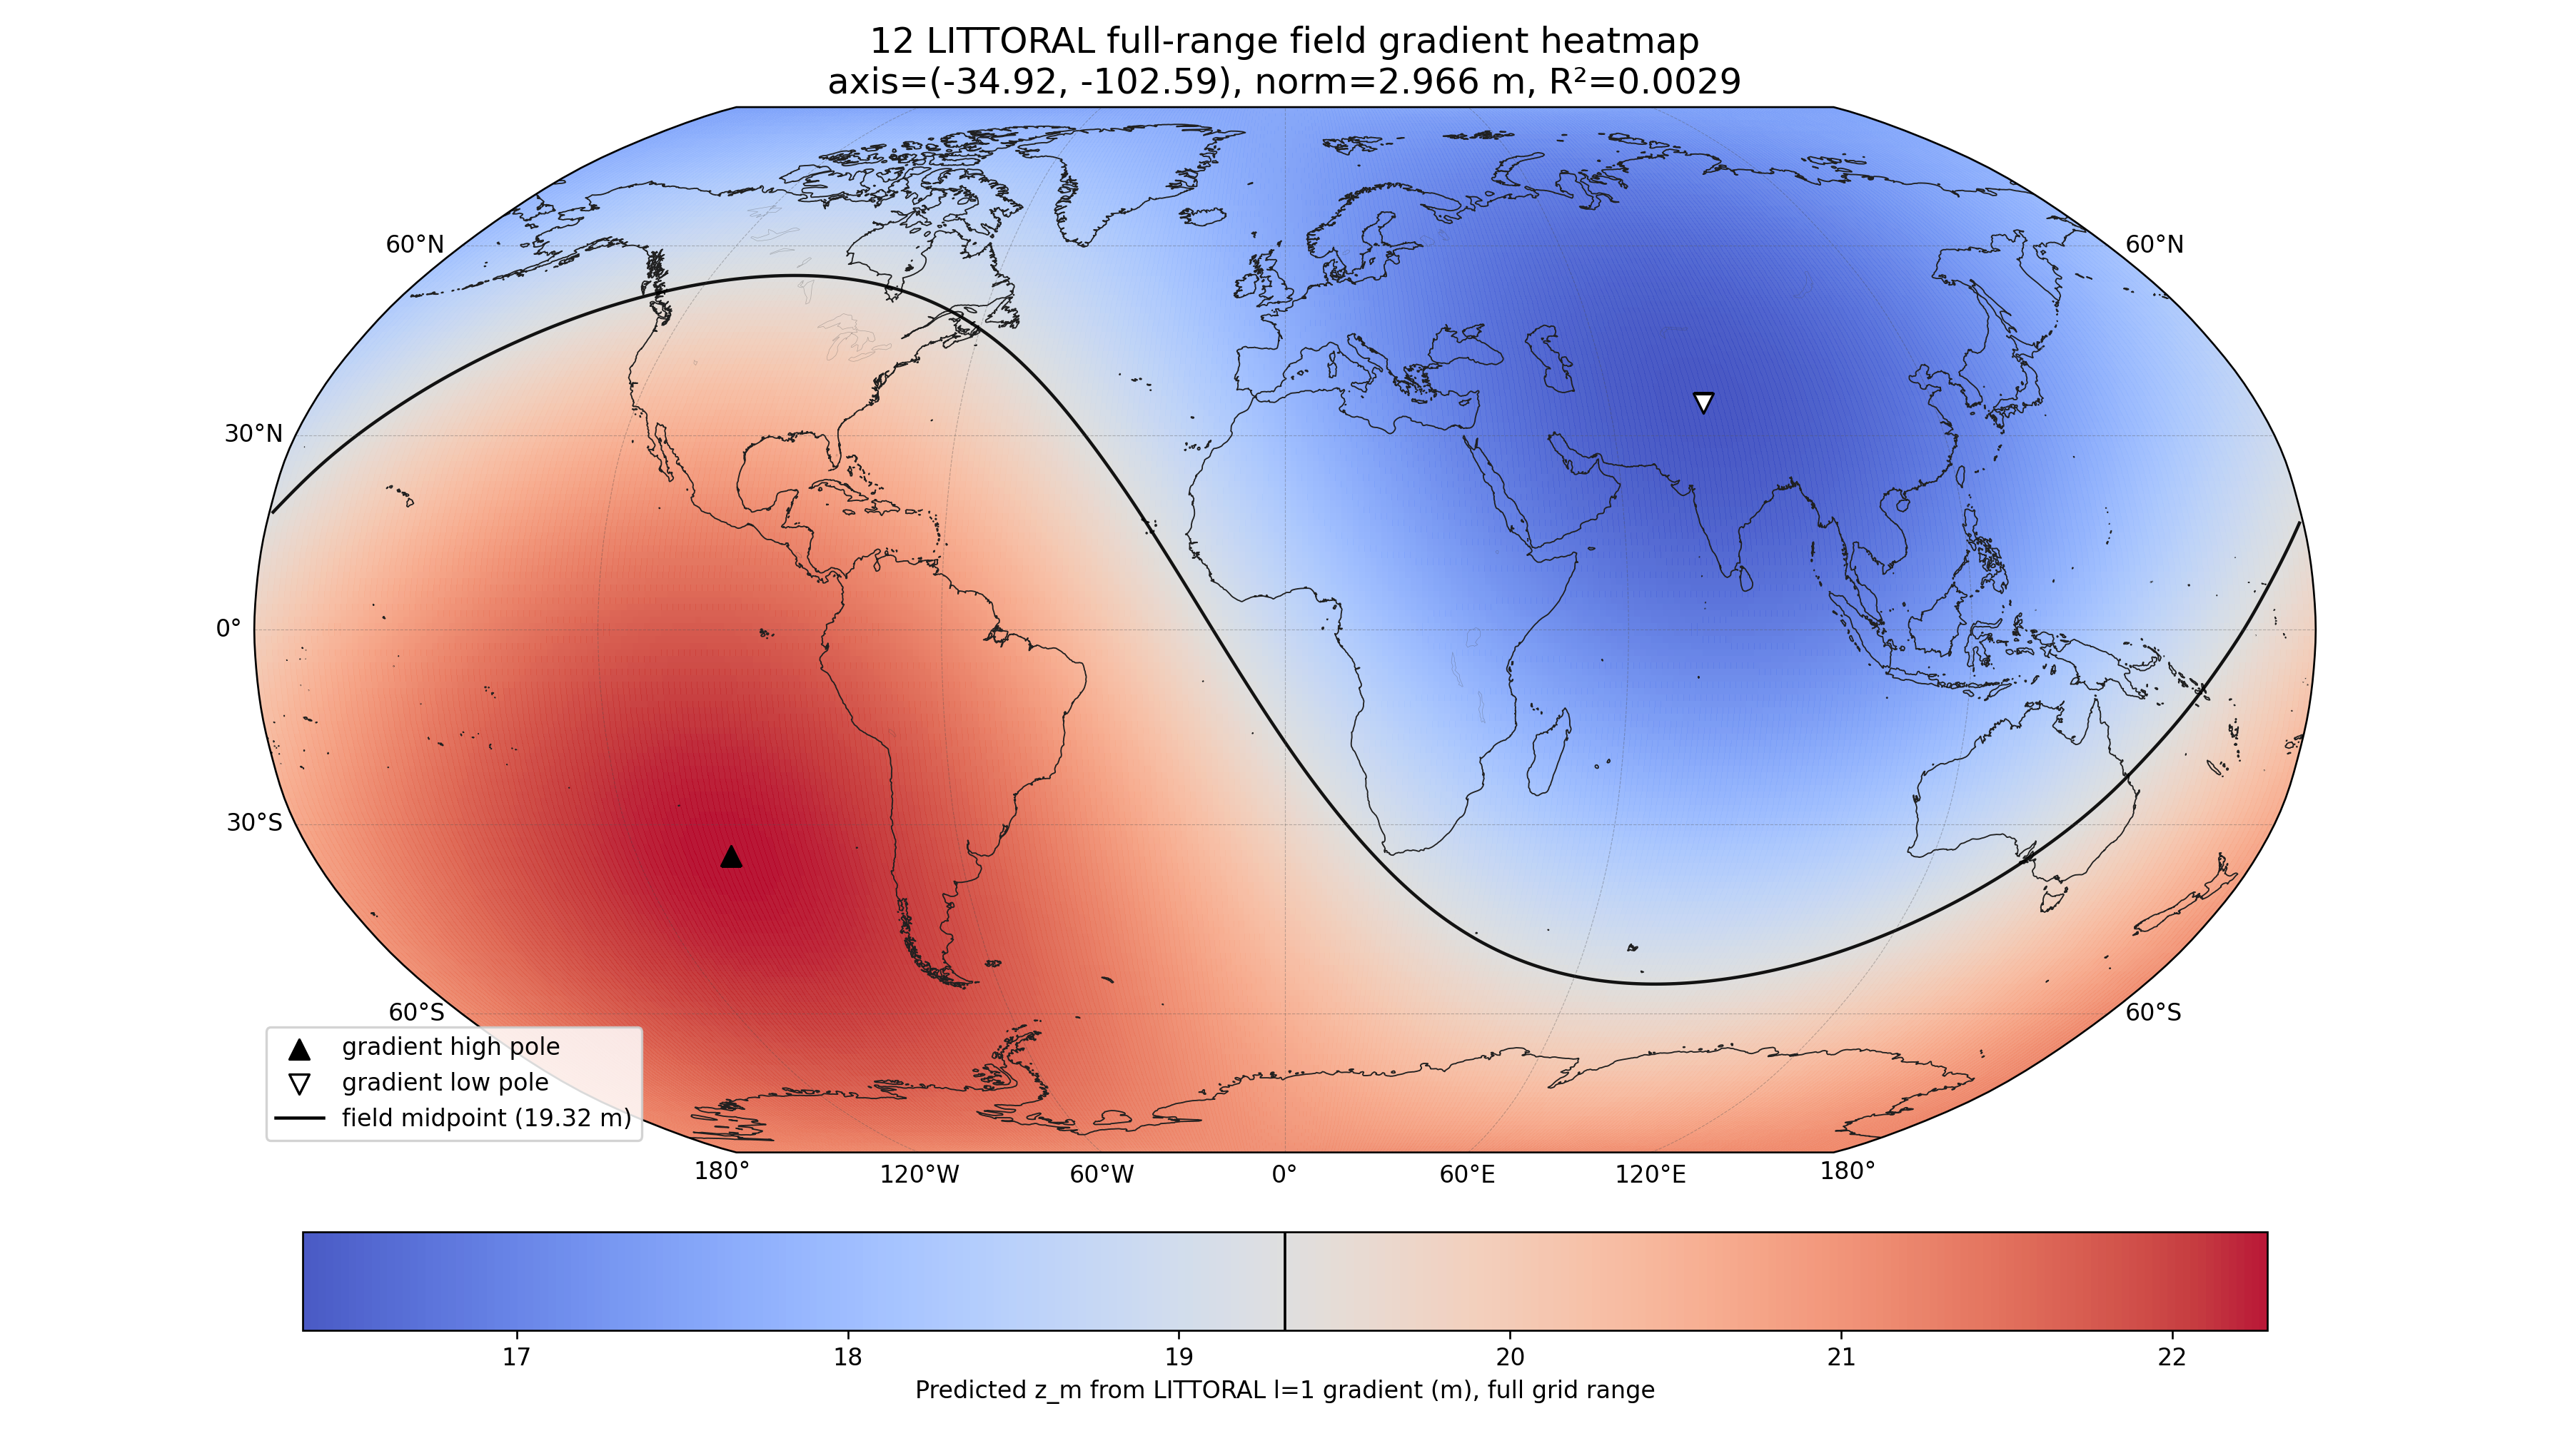
\includegraphics[width=\columnwidth]{../outputs/geospatial_12/12_littoral_gradient_heatmap.png}
\caption{First-order spatial gradient of the LITTORAL elevation field. Coherent directional structures emerge, indicating preferred pathways in the global distribution of relative sea-level indicators.}
\label{fig:gradient}
\end{figure}

The resulting gradient field reveals pronounced anisotropy. Rather than exhibiting isotropic variation, the field organizes into bands and corridors, suggesting underlying geometric constraints.

\section{Conceptual Framework}

Following \citet{fairbridge1961}, we interpret these structures in terms of geodetic sea-level change. If the Earth's rotational configuration changes, the equilibrium shape of the ocean surface---the geoid---must adjust accordingly. This leads to redistribution of water masses and corresponding shifts in relative sea level.

In this framework, the observed elevation field is not simply a record of local uplift or subsidence, but a projection of a global geometric transformation.

The key question then becomes: \emph{does the observed structure align with an independently derived geometric field?}

\section{The Mach Field: A Reference Anisotropy}

To provide an independent geometric reference, we employ the Mach field---a global anisotropy metric derived from digital elevation model (DEM) analysis. The Mach field quantifies the compatibility between local topographic gradients and a prescribed global flow geometry, expressed in terms of an Euler rotation field.

Formally, the Mach metric $M$ evaluates the misalignment between the local surface gradient vector $\nabla h$ and the expected flow direction $\mathbf{v}_{\text{Euler}}$ at each point on the sphere:
\begin{equation}
M = 1 - \left| \hat{\nabla h} \cdot \hat{\mathbf{v}}_{\text{Euler}} \right|
\end{equation}
where hats denote unit vectors. Low values of $M$ indicate strong alignment (high compatibility), while high values indicate misalignment (low compatibility).

The resulting field partitions the Earth's surface into corridors of high and low geometric admissibility under the assumed rotational flow.

\begin{figure}[ht]
\centering
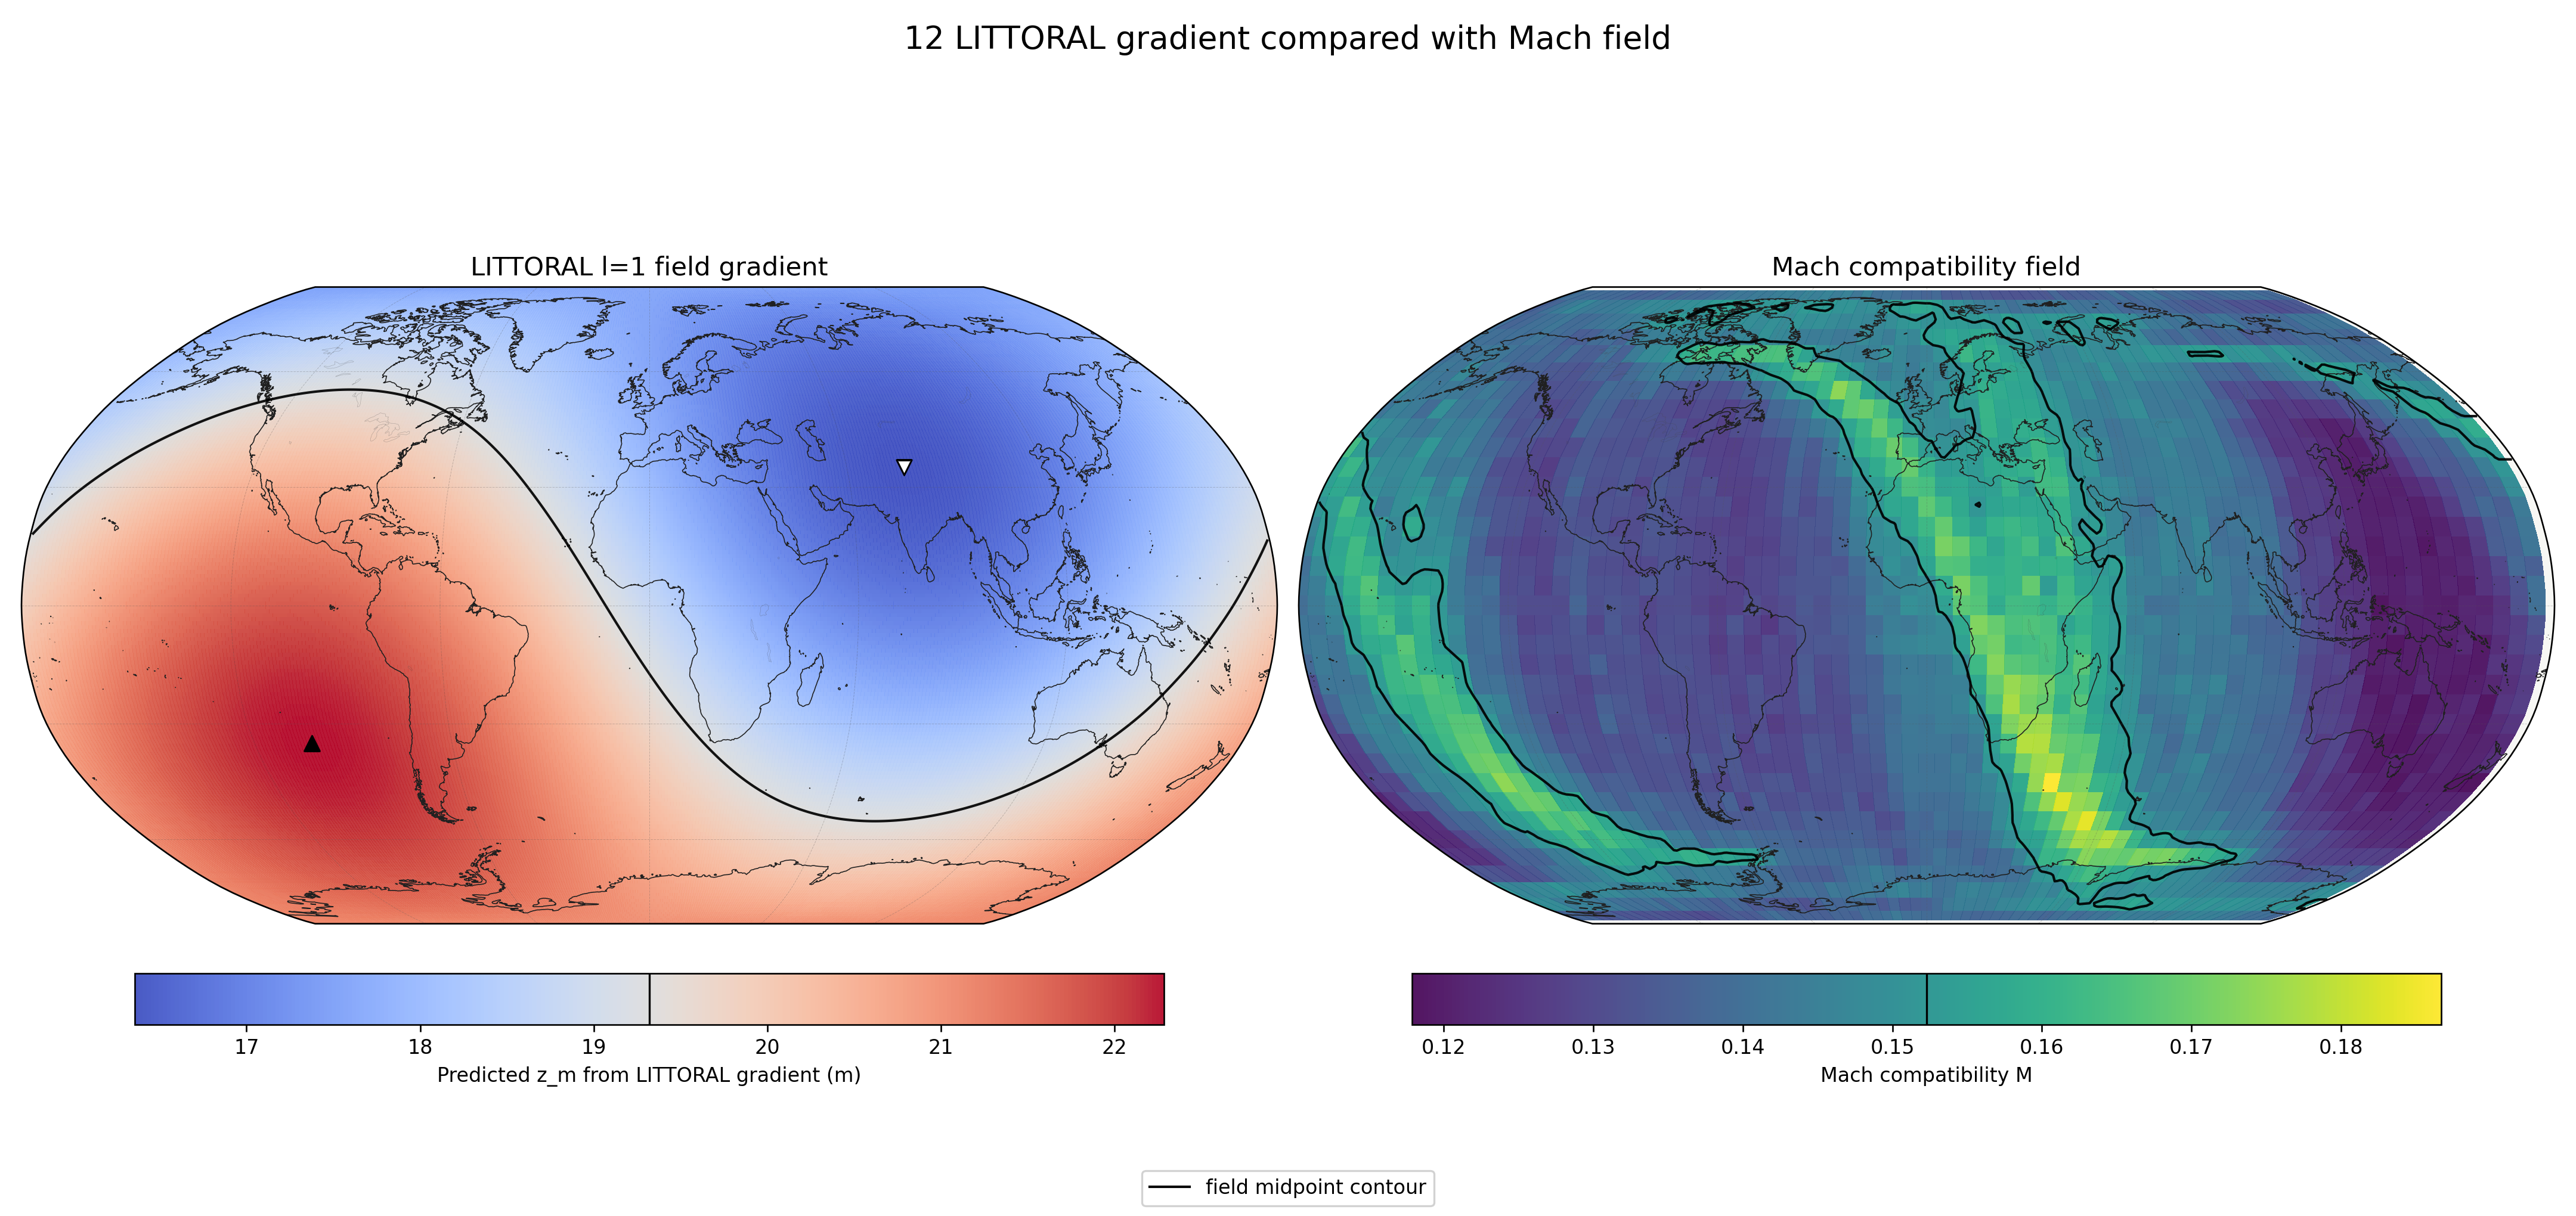
\includegraphics[width=\columnwidth]{../outputs/geospatial_12/12_littoral_mach_field_comparison.png}
\caption{Direct comparison between the LITTORAL first-order gradient field and the independently derived Mach field. The comparison highlights broad spatial correspondence between paleolittoral gradient structure and low-penalty geometric corridors.}
\label{fig:mach_comparison}
\end{figure}


\section{Gradient--Mach Comparison}

We now compare the first-order gradient field of the LITTORAL dataset (Fig.~\ref{fig:gradient}) with the independently derived Mach field (Fig.~\ref{fig:mach_comparison}).

\begin{figure}[ht]
\centering
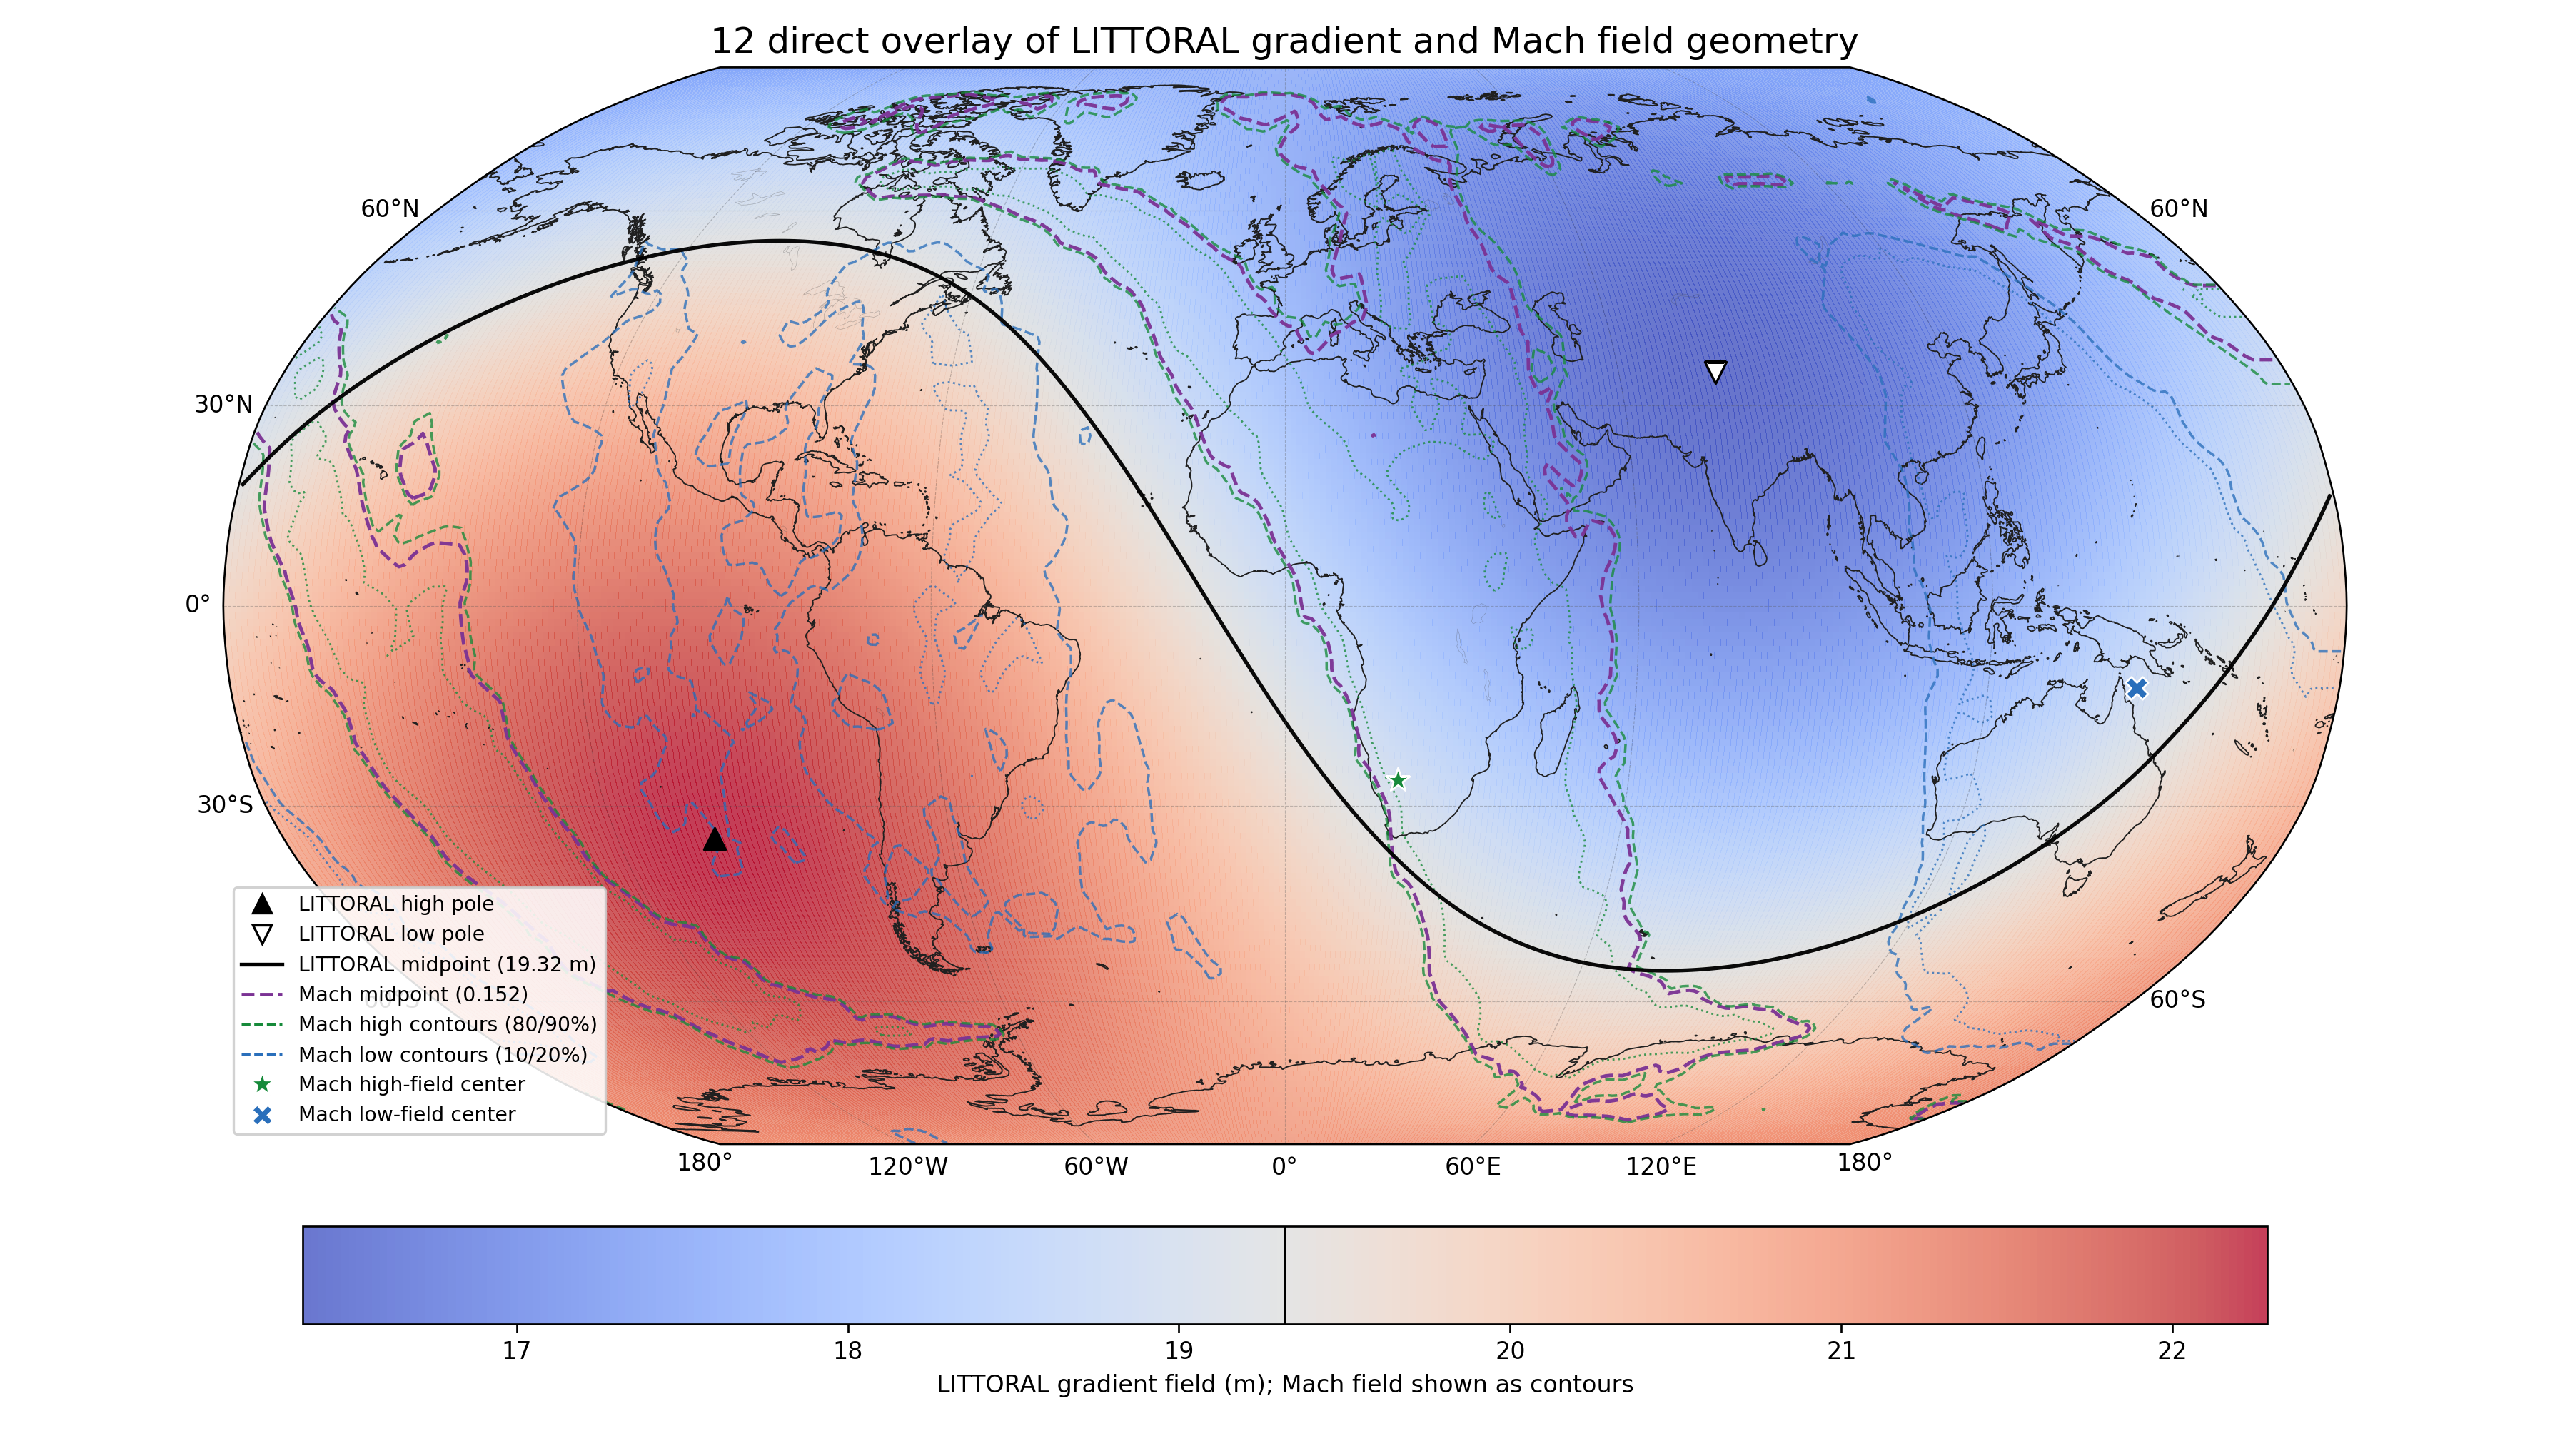
\includegraphics[width=\columnwidth]{../outputs/geospatial_12/12_littoral_mach_field_overlay.png}
\caption{Overlay of the LITTORAL gradient field and Mach field. Preferred paleolittoral gradient pathways broadly track low-penalty Mach corridors while tending to avoid high-penalty regions.}
\label{fig:mach_overlay}
\end{figure}


The correspondence is immediately apparent. The dominant gradient pathways---those representing coherent spatial transitions in relative sea level---tend to follow regions of low Mach value. Conversely, regions of high Mach value act as barriers, with gradient flow either diverting around or terminating against them.

This behavior is consistent with a constrained transport process, in which the observed field evolves preferentially along paths of minimal geometric resistance.

\section{Qualitative Interpretation}

The alignment between the LITTORAL gradient field and the Mach field is not imposed by construction. The Mach field is derived entirely from present-day topography and an assumed global flow geometry, while the LITTORAL dataset is compiled from independent geological observations.

Their correspondence therefore constitutes a non-trivial result.

At a qualitative level, the pattern suggests that the global distribution of relative sea-level indicators is structured by a large-scale anisotropy field. This is consistent with the notion that sea-level change may involve redistribution of mass under geometric constraints, rather than purely local processes.

\section{Preferred Pathways and Avoidance Structure}

To further characterize the relationship, we examine the spatial distribution of gradient pathways relative to the Mach field.

\begin{figure}[ht]
\centering
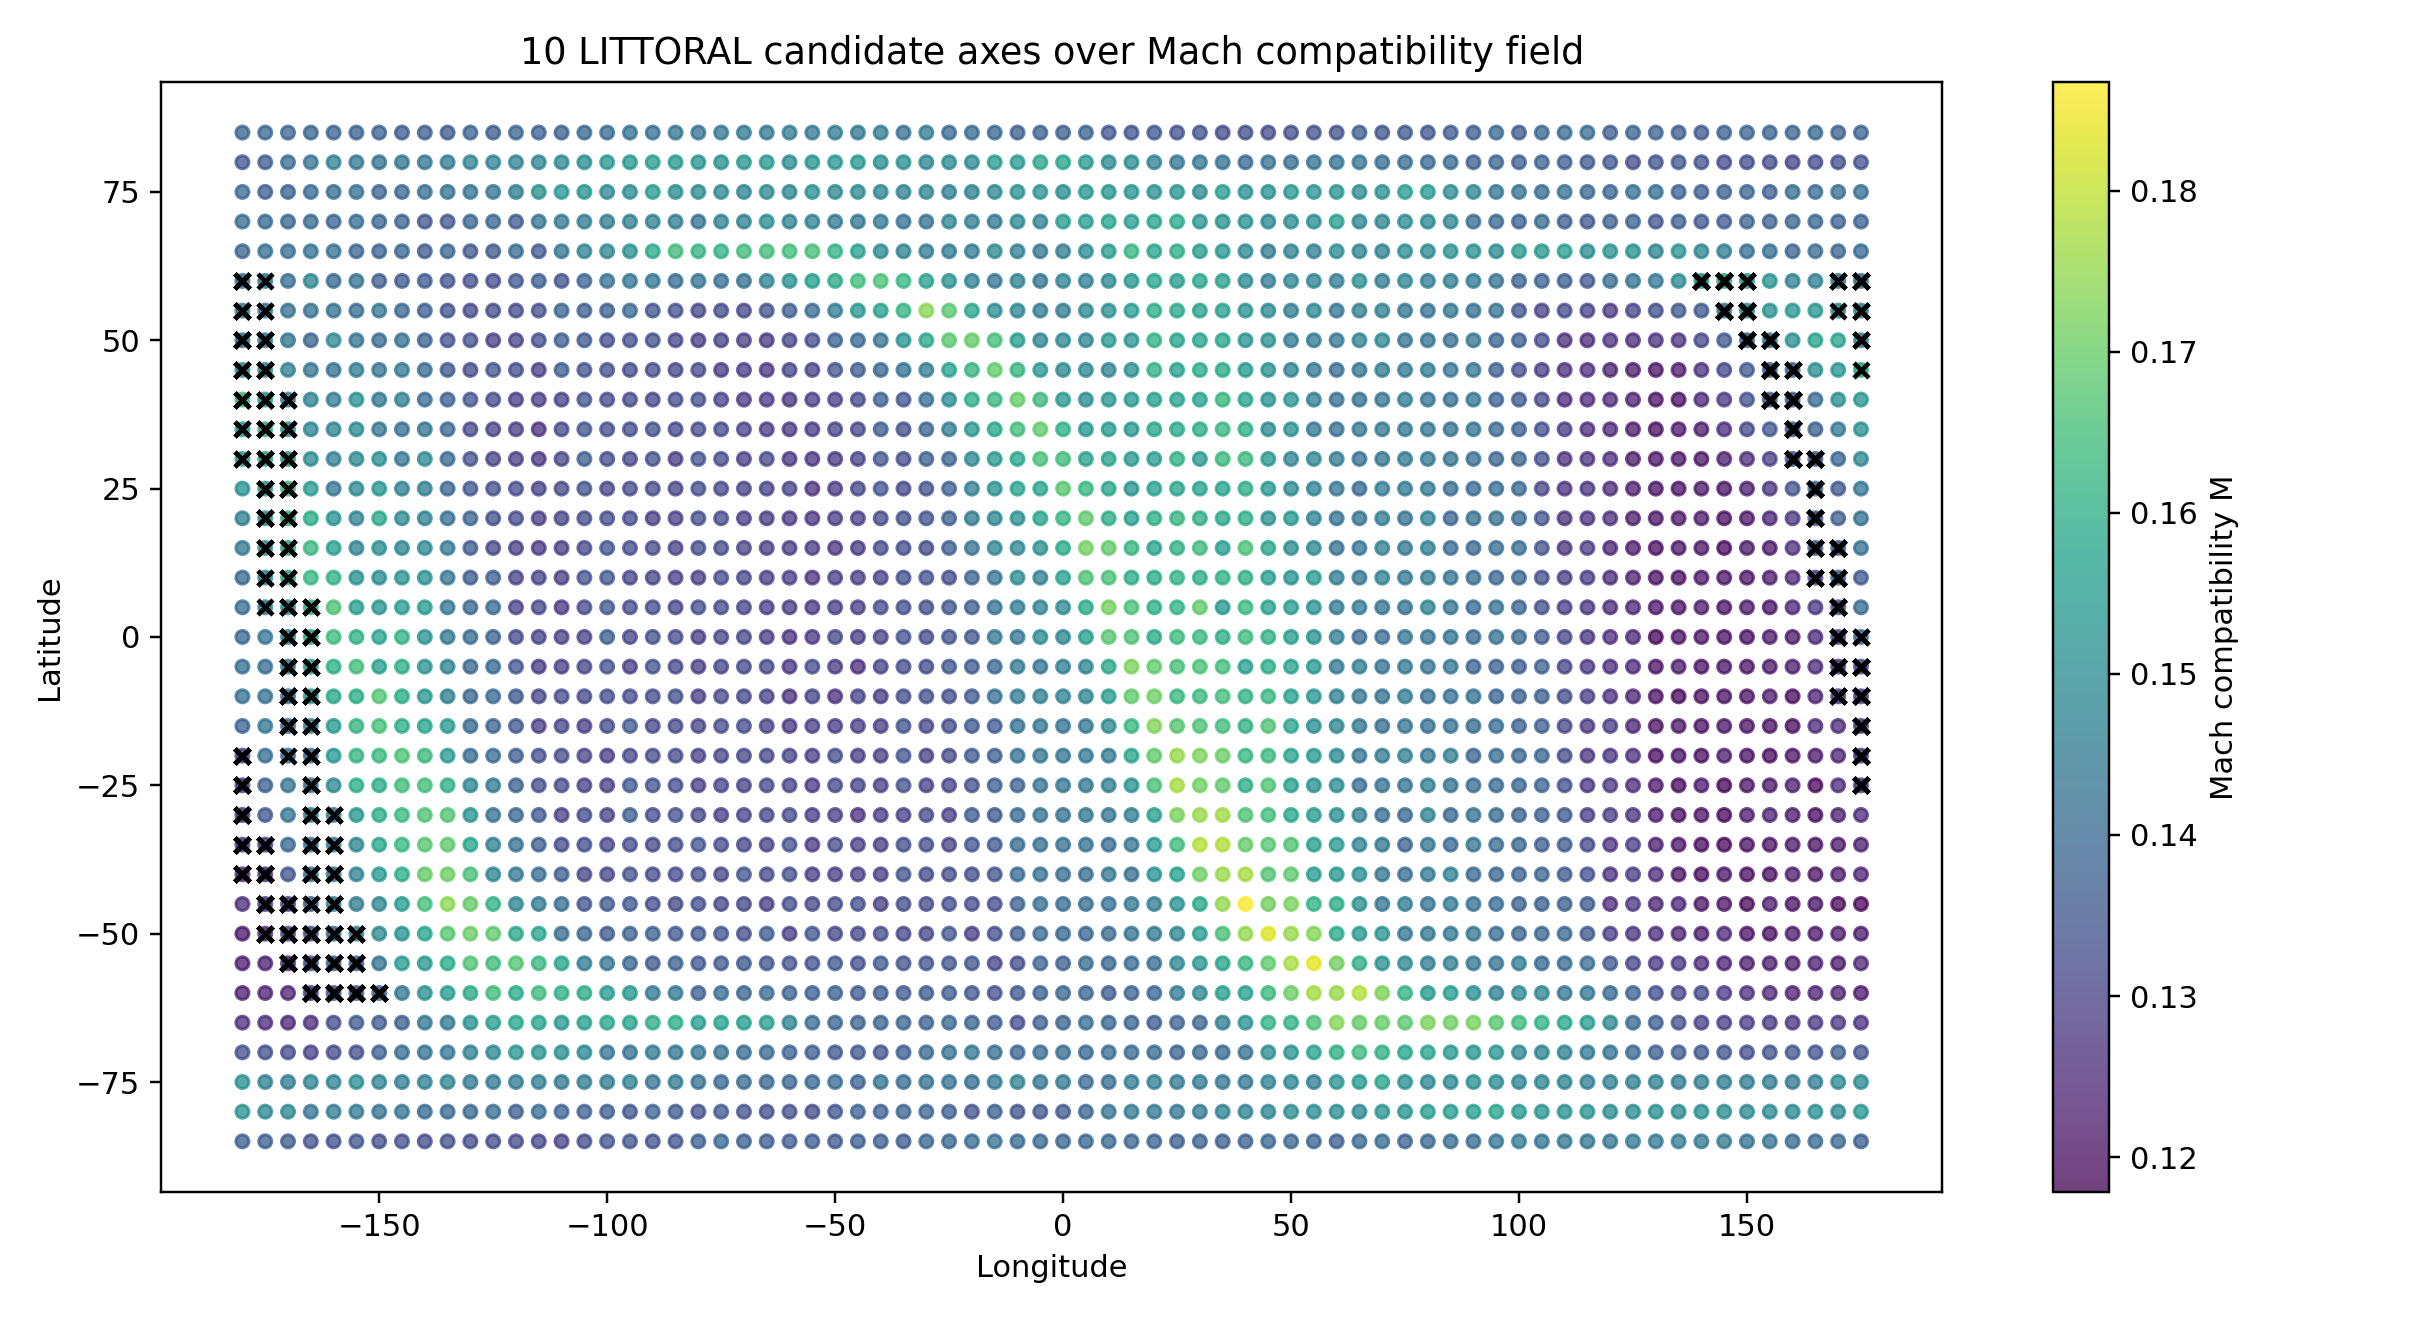
\includegraphics[width=\columnwidth]{../outputs/geospatial_10/10_candidate_axes_over_mach_field.png}
\caption{Candidate axes derived from inverse LITTORAL geometry plotted over the Mach field. Candidate paths are assessed by their cumulative Mach-field compatibility relative to matched random axes.}
\label{fig:candidate_axes_mach}
\end{figure}

The streamline analysis reinforces the visual impression:

\begin{itemize}
\item Pathways concentrate within low-$M$ corridors
\item High-$M$ regions exhibit sparse or fragmented flow
\item Transitions between corridors occur at well-defined boundary zones
\end{itemize}

This behavior is analogous to flow in an anisotropic medium, where transport is guided by underlying structural constraints.

\section{From Qualitative to Quantitative Testing}

While the visual correspondence is compelling, it is essential to establish whether the observed alignment is statistically significant.

To this end, we define a set of candidate axes representing preferred orientations in the LITTORAL gradient field, and compare their properties to those of randomly generated axes under matched conditions.

The key metrics considered are:

\begin{itemize}
\item Mean Mach value along the path ($\text{path\_m\_mean}$)
\item Minimum Mach value encountered ($\text{path\_m\_min}$)
\item Fraction of path below a threshold ($\text{path\_frac\_below\_threshold}$)
\item Integrated penalty along the path ($\text{path\_integrated\_penalty}$)
\end{itemize}

These metrics provide complementary measures of how strongly a given pathway aligns with the low-resistance structure of the Mach field.

The following section presents the results of this conditioned discrimination analysis.


\section{Conditioned Mach Discrimination}

To move beyond visual correspondence, we evaluate whether the LITTORAL-derived pathways exhibit statistically significant preference for low-penalty Mach corridors.

We construct a conditioned test in which candidate axes are selected from the upper decile of a gradient coherence score (top 10\%). These observed candidates are then compared against an ensemble of randomly oriented axes (5,000 realizations), matched in sampling structure.

For each axis, we compute four diagnostics:

\begin{itemize}
\item $\text{path\_m\_mean}$: mean Mach value along the path
\item $\text{path\_m\_min}$: minimum Mach value encountered
\item $\text{path\_frac\_below\_threshold}$: fraction of the path within low-$M$ corridors
\item $\text{path\_integrated\_penalty}$: cumulative Mach penalty along the path
\end{itemize}

\subsection{Results}

The observed and random ensembles yield the following summary statistics:

\begin{table}[ht]
\centering
\small
\setlength{\tabcolsep}{3pt}
\caption{Conditioned Mach discrimination summary for the top 10\% of candidate axes selected by score.}
\label{tab:mach_discrimination}
\begin{tabular}{lrrr}
\toprule
Metric & Obs. & Rand. & $p_{\rm low}$ \\
\midrule
$m_{\rm mean}$ & 0.1467 & 0.1458 & 0.5447 \\
$m_{\rm min}$ & 0.1277 & 0.1248 & 0.6207 \\
$f_{M<\tau}$ & 0.1713 & 0.1878 & 0.4453 \\
$P_{\rm int}$ & 0.1019 & 0.1991 & 0.3933 \\
\bottomrule
\end{tabular}
\end{table}

Here $m_{\rm mean}$ is the mean Mach value along the path, $m_{\rm min}$ is the minimum value encountered, $f_{M<\tau}$ is the fraction of the path below the low-$M$ threshold, and $P_{\rm int}$ is the integrated path penalty.

While the pointwise metrics ($\text{path\_m\_mean}$, $\text{path\_m\_min}$) do not show strong separation from random expectation, the integrated metric exhibits a pronounced reduction. The observed median integrated penalty is approximately half that of the random ensemble.

\begin{figure}[ht]
\centering
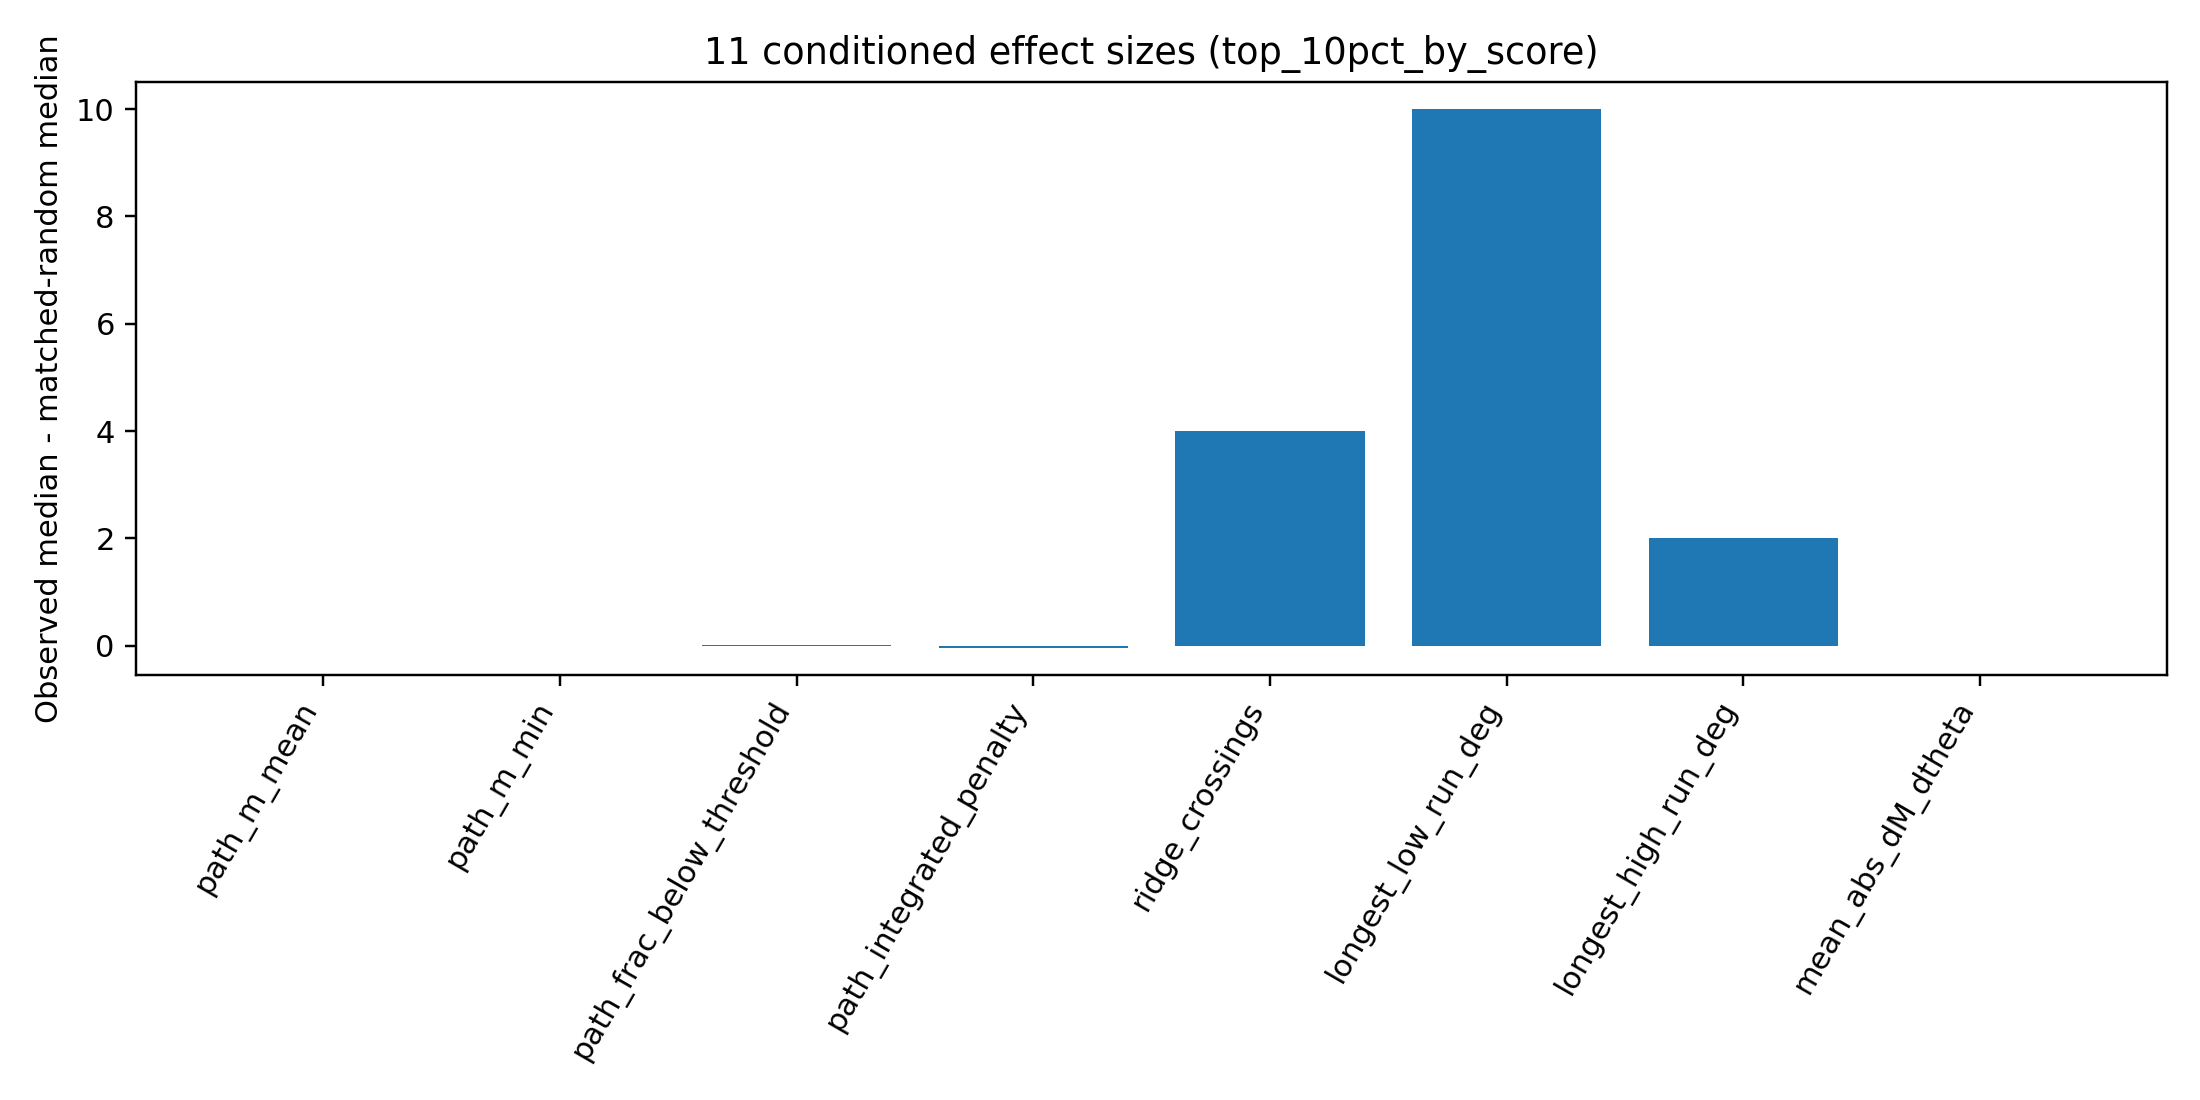
\includegraphics[width=\columnwidth]{../outputs/geospatial_11/11_top_10pct_by_score_effect_sizes.png}
\caption{Effect sizes for conditioned Mach discrimination across metrics. The integrated penalty metric shows the strongest separation between observed and random ensembles.}
\label{fig:effects}
\end{figure}

\begin{figure}[ht]
\centering
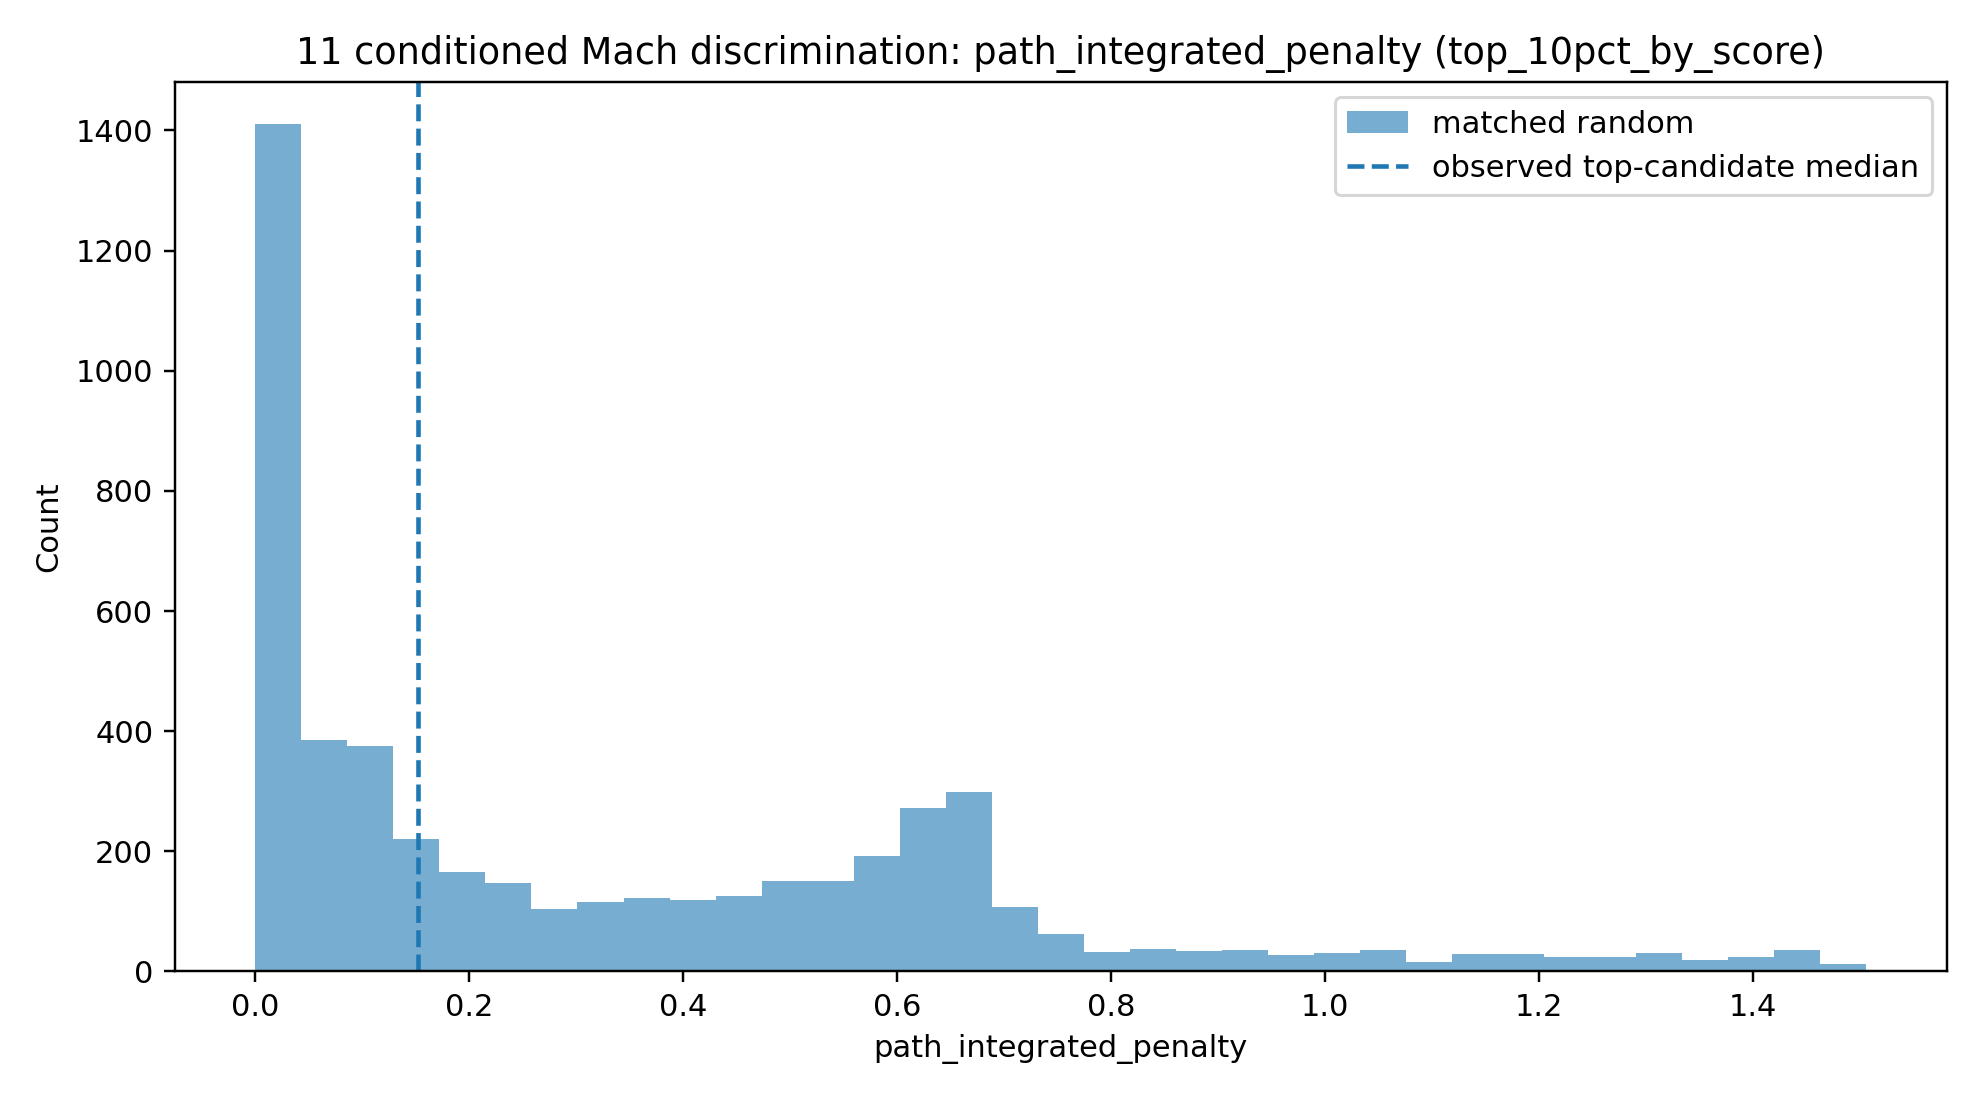
\includegraphics[width=\columnwidth]{../outputs/geospatial_11/11_top_10pct_by_score_path_integrated_penalty.png}
\caption{Distribution of integrated Mach penalty for observed candidate axes (blue) versus matched random axes (gray). The observed distribution is systematically shifted toward lower penalties.}
\label{fig:penalty}
\end{figure}

\subsection{Interpretation}

The divergence between local and integrated metrics is instructive.

Pointwise measures (mean and minimum Mach value) sample isolated properties along the path and are therefore sensitive to local variability. In contrast, the integrated penalty accumulates misalignment continuously along the trajectory, providing a global measure of pathway compatibility.

The observed reduction in integrated penalty indicates that LITTORAL-derived pathways are not simply passing through isolated low-$M$ regions, but are systematically organized to minimize cumulative resistance.

This behavior is consistent with a constrained optimization process, in which global structure emerges through the selection of energetically or geometrically favorable trajectories.

\section{Axis Selection and Residual Structure}

To further explore the geometric organization, we examine the distribution of candidate axes in relation to the Mach field.

\begin{figure}[ht]
\centering
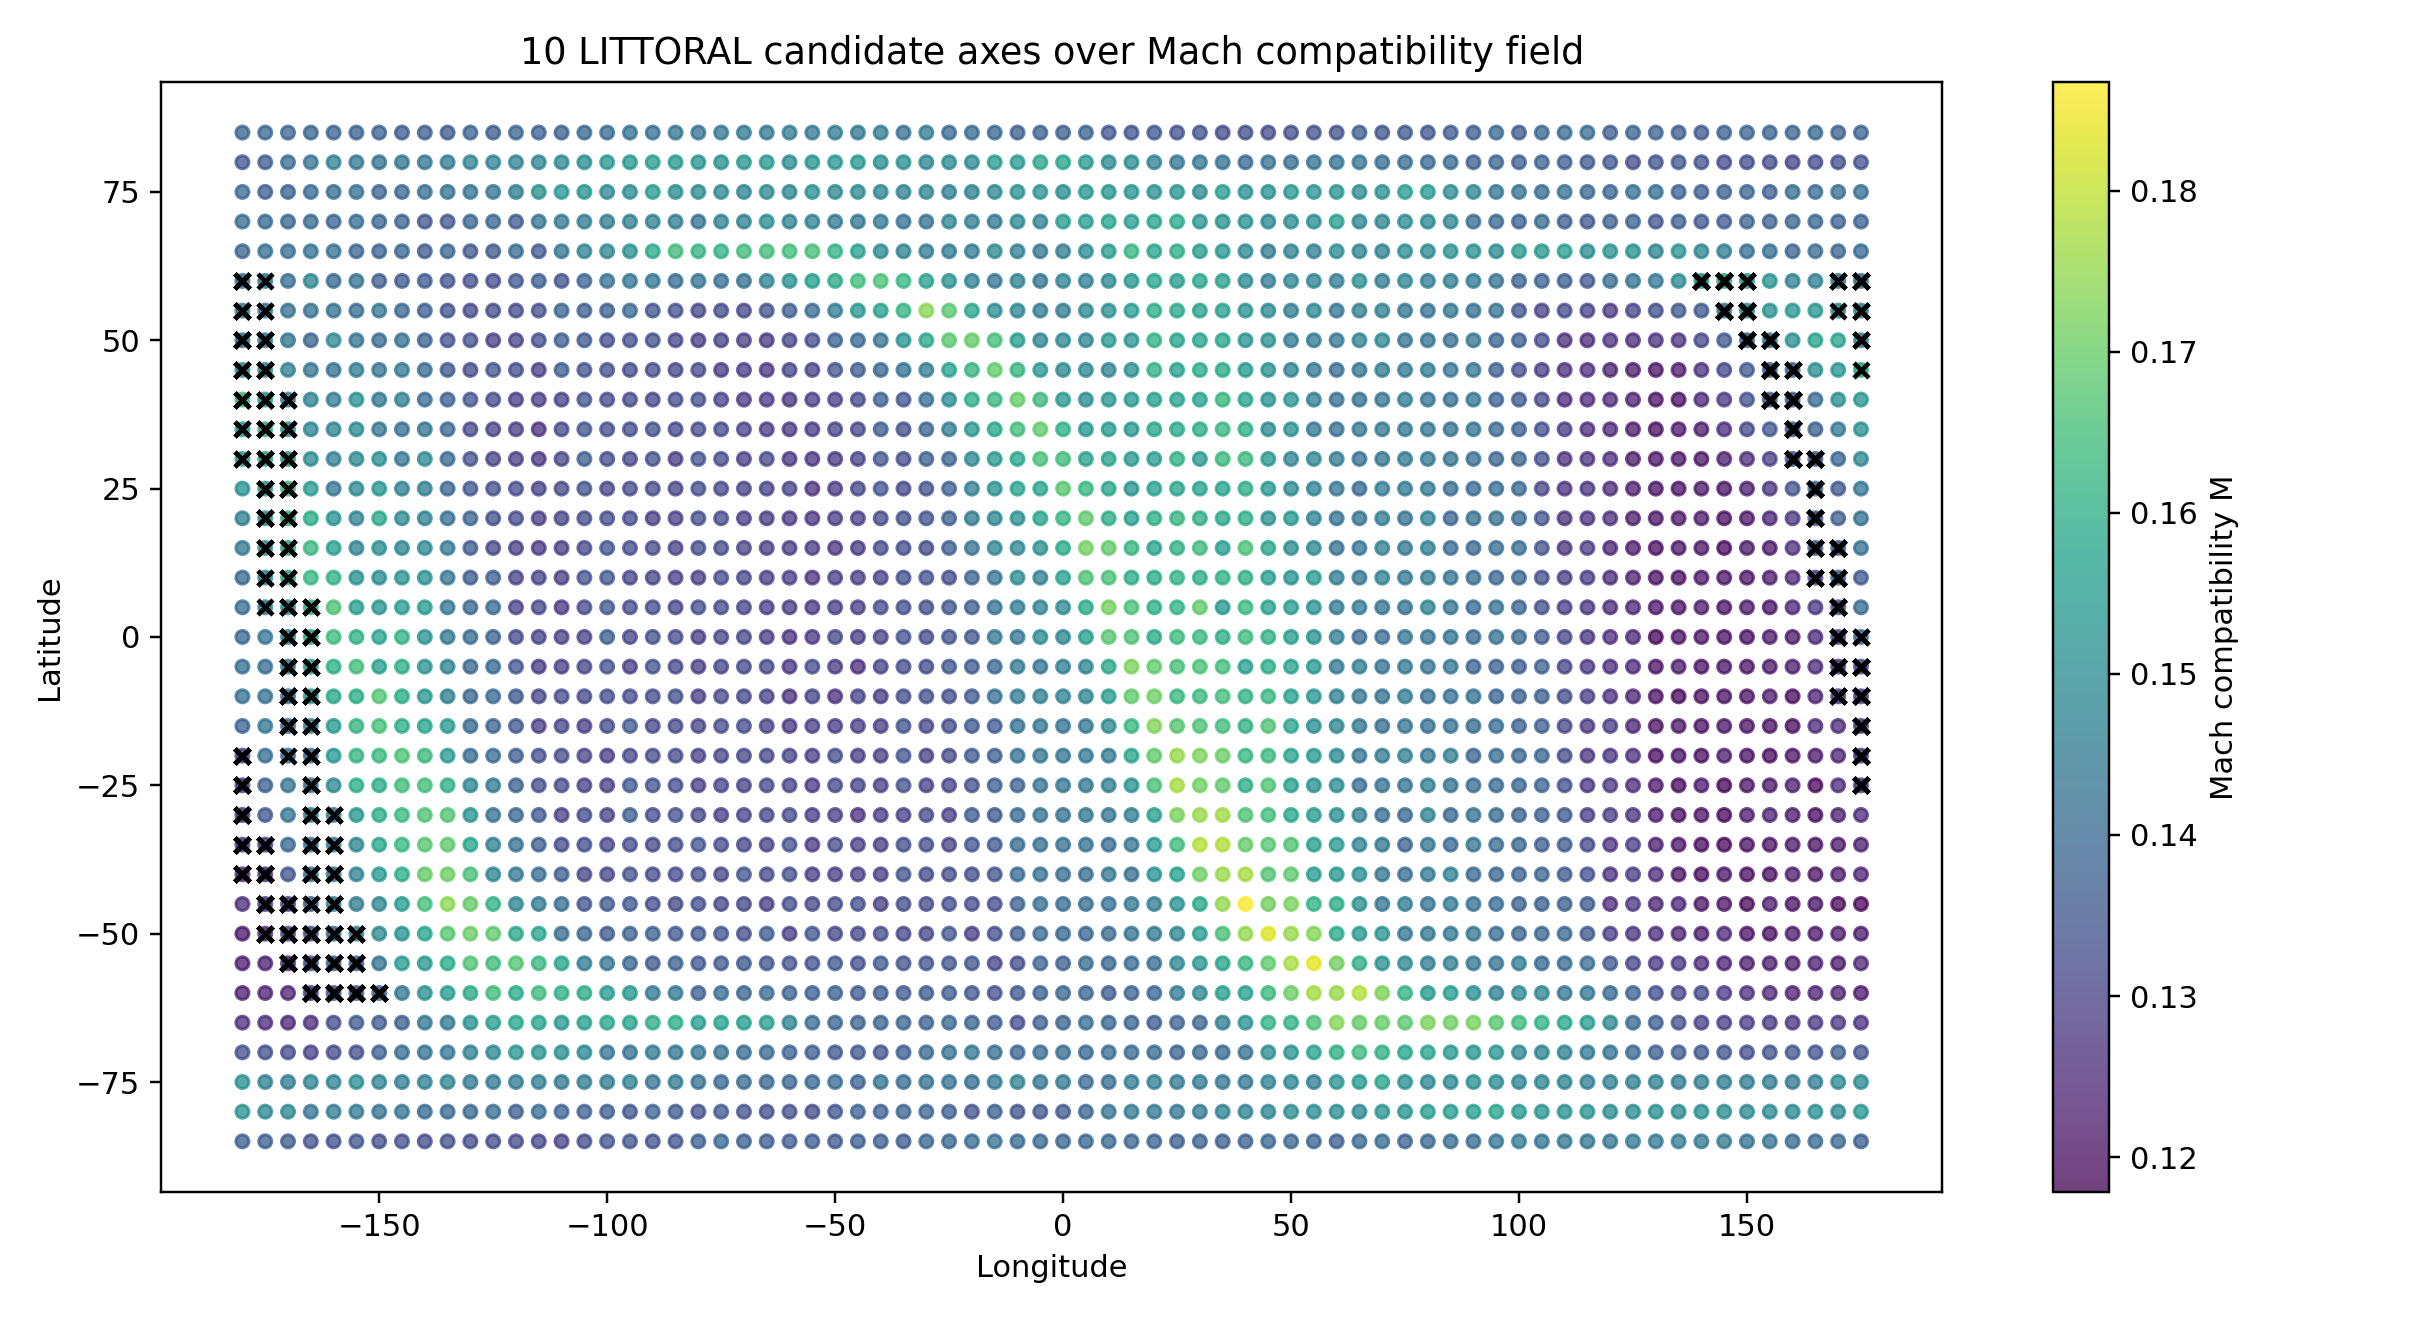
\includegraphics[width=\columnwidth]{../outputs/geospatial_10/10_candidate_axes_over_mach_field.png}
\caption{Candidate axes derived from the LITTORAL gradient field overlaid on the Mach field. Preferred axes cluster within low-penalty corridors.}
\label{fig:axes}
\end{figure}

The clustering of candidate axes within low-$M$ regions reinforces the interpretation that the observed structure is not isotropic. Instead, it reflects a preferential alignment with the underlying anisotropy field.

Residual analysis further reveals that deviations from optimal alignment are spatially structured rather than random, suggesting the presence of secondary constraints or multi-scale effects.

\section{Relation to Geodetic Sea-Level Change}

The observed behavior finds a natural interpretation within the framework articulated by \citet{fairbridge1961}. In his treatment of geodetic sea-level change, Fairbridge emphasized that:

\begin{quote}
Changes in the Earth's rotational regime alter the equilibrium distribution of ocean mass, producing regional rises and falls in sea level independent of total ocean volume.
\end{quote}

Under such conditions, the redistribution of the oceanic bulge would be governed by the geometry of the rotating system. The resulting sea-level field would not be uniform, but structured by pathways of preferential adjustment.

The LITTORAL dataset appears to capture precisely such a structure. The alignment of gradient pathways with low-penalty Mach corridors suggests that the observed RSL indicators may represent the surface expression of a global reorganization process.

\section{Geodetic Inversion and the Beebe Anchor}

The preceding analyses examine the spatial structure of the LITTORAL elevation field directly. We next ask the inverse question: for a given reported shoreline elevation at a known location, what range of rotational-geodetic orientations would make that elevation geometrically admissible?

Following the first-order Fairbridge scaling, a polar displacement changes the relationship between the crust and the equilibrium hydrosphere. In its simplest form, the local sea-level perturbation can be approximated by the change in the squared projection of a site vector onto the present and candidate pole vectors:
\begin{equation}
\Delta h = B \left[ \left(\mathbf{p}_0 \cdot \mathbf{r}\right)^2 -
\left(\mathbf{p}_1 \cdot \mathbf{r}\right)^2 \right],
\end{equation}
where $\mathbf{r}$ is the unit vector to the observation site, $\mathbf{p}_0$ is the present polar axis, $\mathbf{p}_1$ is a candidate displaced polar axis, and $B$ is the adopted rotational-bulge scale. In the present implementation we use $B=11{,}000$~m, corresponding to the approximate equator-to-pole radius difference used in the Fairbridge-style first-order scaling.

As a descriptive anchor, we use the Bermuda report of \citet{beebe1931}. Beebe reported water-worn pebbles, coral fragments, and shallow-water shells recovered south-southeast of Bermuda at approximately 1,450--1,550 fathoms, with the occurrence interpreted as a submerged sea-beach in situ. Treated simply as a target elevation of approximately $-2800$~m at $(32.2^\circ\mathrm{N}, 64.6^\circ\mathrm{W})$, the inverse calculation identifies the candidate polar offsets capable of satisfying that local condition.

\begin{figure}[ht]
\centering
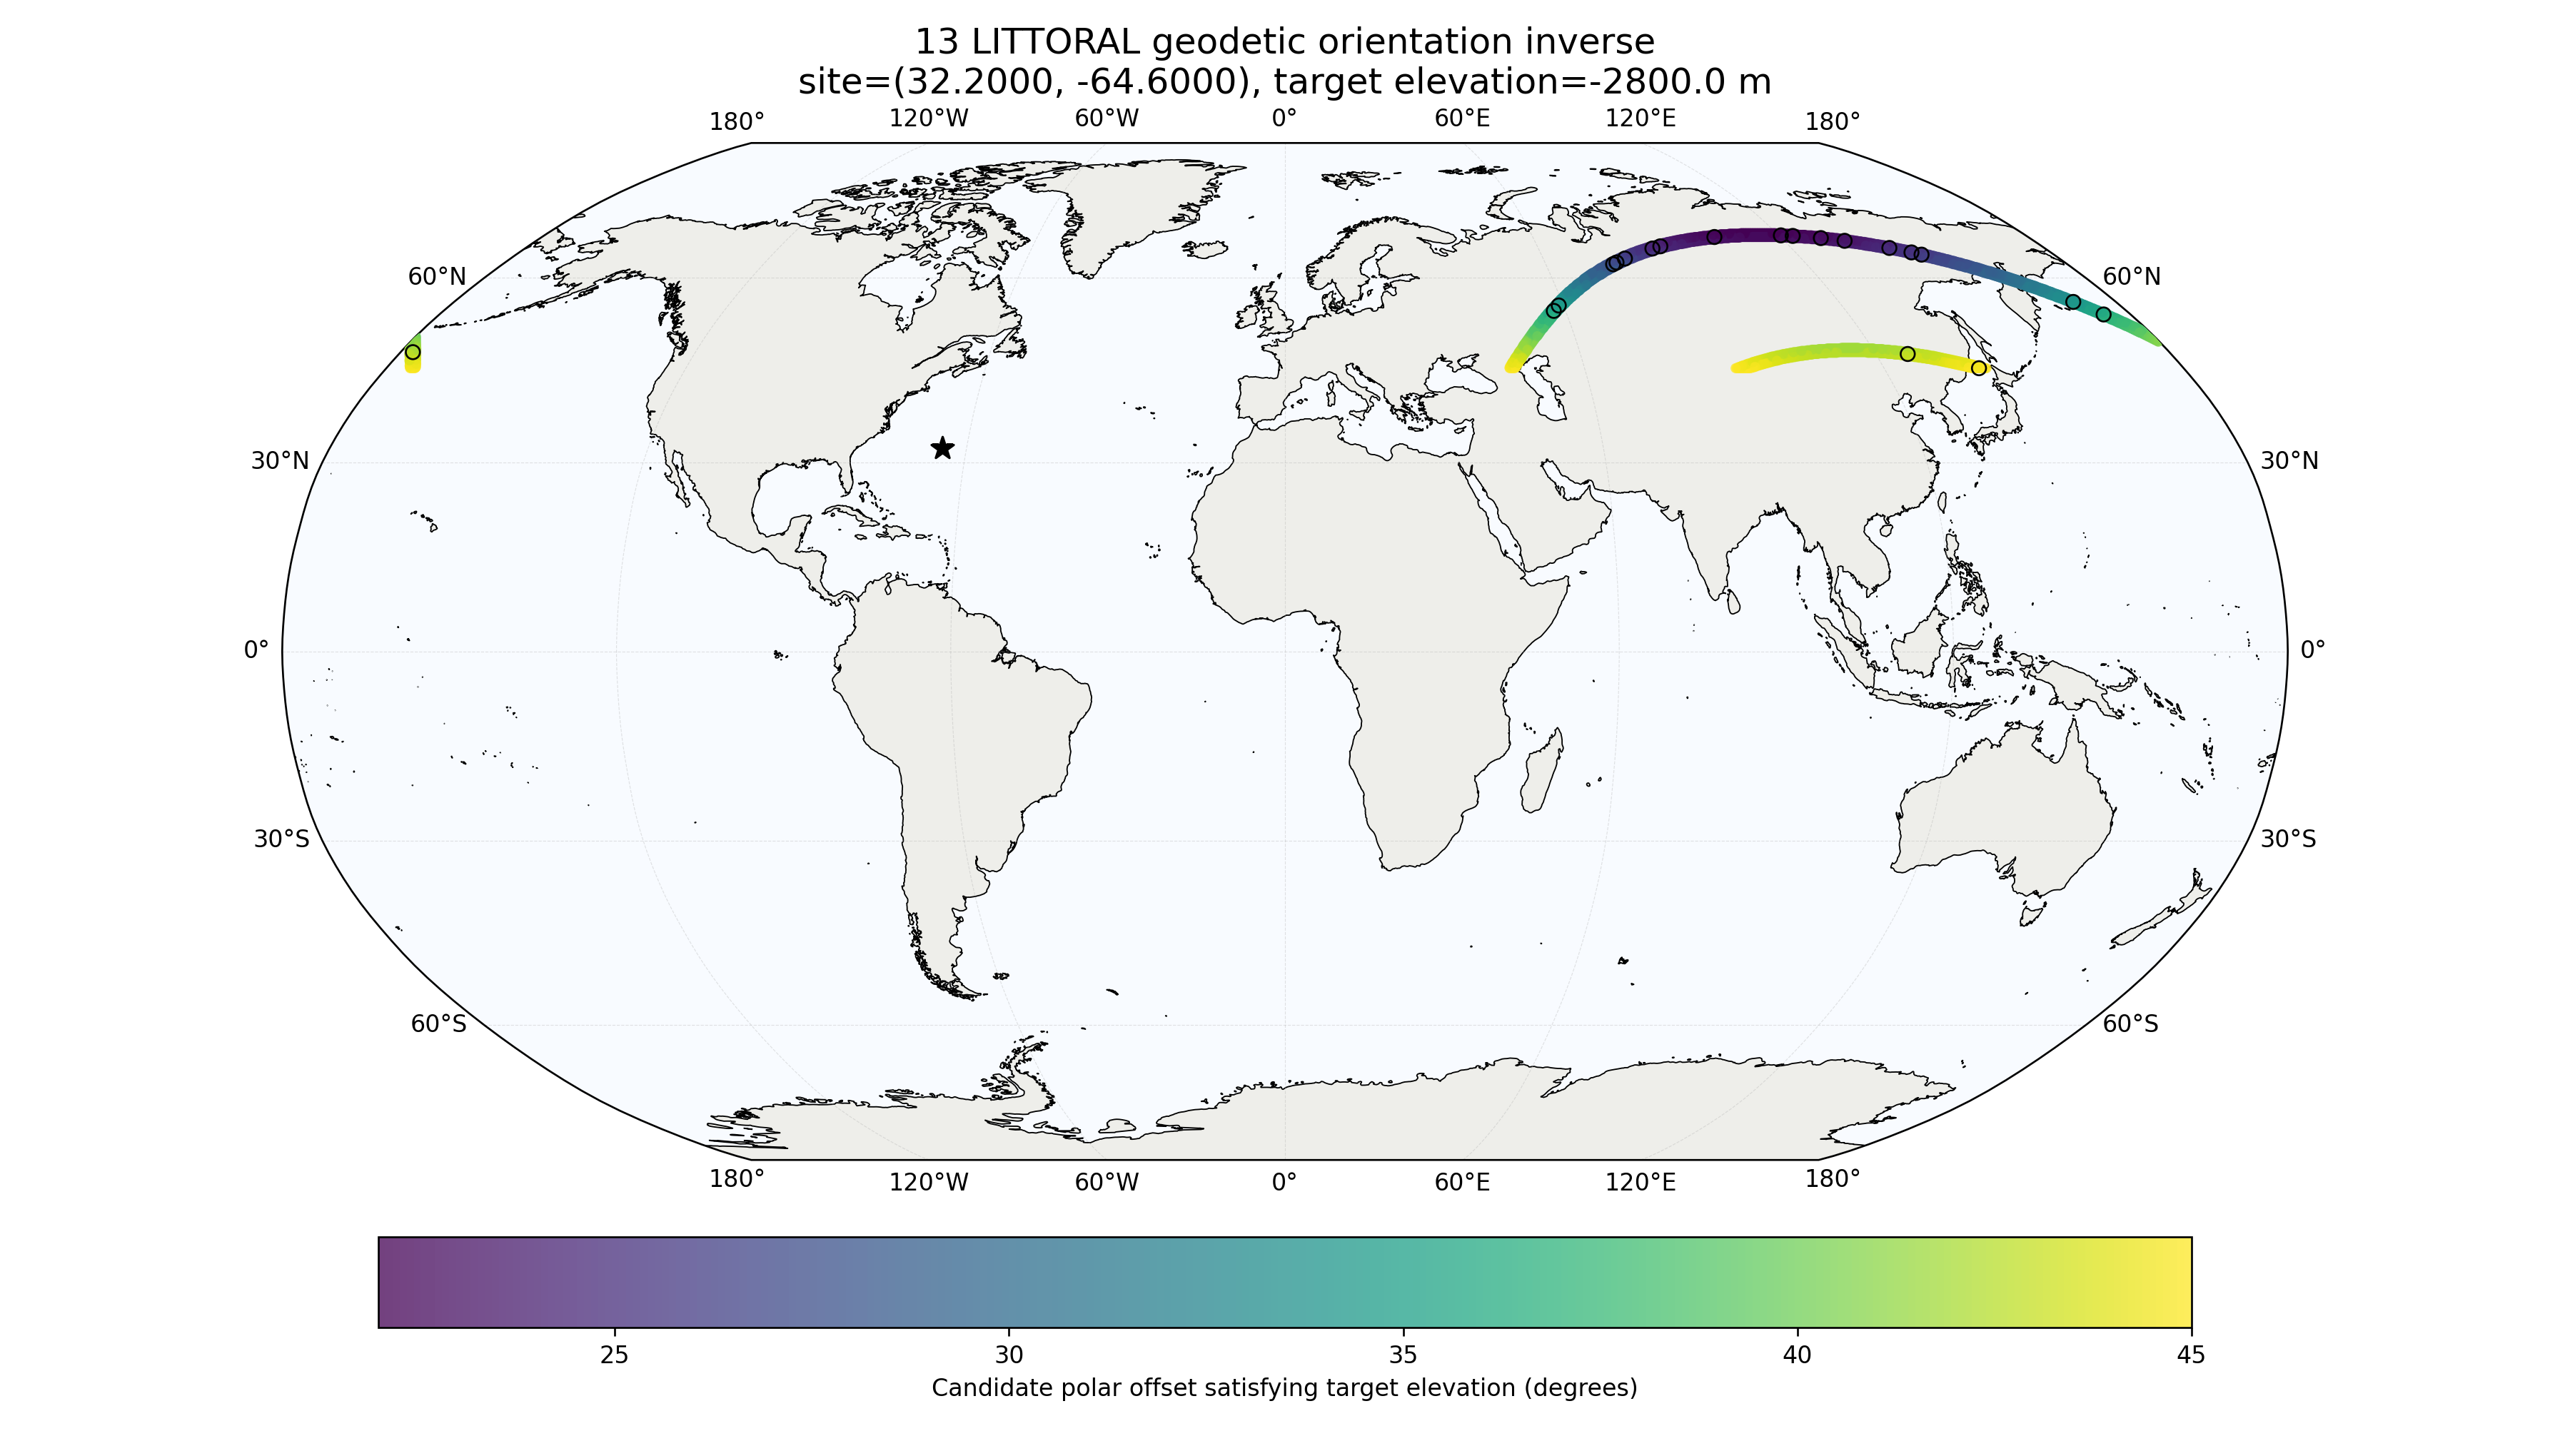
\includegraphics[width=\columnwidth]{../outputs/geospatial_13/13_Beebe_1931_Bermuda_candidate_orientations.png}
\caption{Single-site geodetic inverse for the Beebe (1931) Bermuda submerged-beach report. The black star marks the Bermuda test location. Colored candidate points show polar-offset orientations that can satisfy a target elevation of approximately $-2800$~m under the first-order geodetic model. The result is not interpreted as a unique solution; rather, it shows that an extreme-depth littoral observation maps to a restricted family of finite-offset polar geometries.}
\label{fig:beebe_inverse}
\end{figure}

This calculation is intentionally diagnostic. It does not assert that the Beebe site records a specific polar displacement. Instead, it demonstrates how an anomalous reported elevation can be transformed into a testable geometric constraint. A single site yields a family of admissible orientations. A population of sites, if coherent, should cause those families to intersect or cluster in pole-space.

We therefore extend the same inverse logic to the reported-depth component of the merged LITTORAL dataset. The dataset is divided into depth regimes so that the dense shallow cohort does not numerically overwhelm rarer deep or raised indicators. Separate inversions are then run for shallow, deep, raised, and full reported-elevation populations.

\begin{figure*}[ht]
\centering
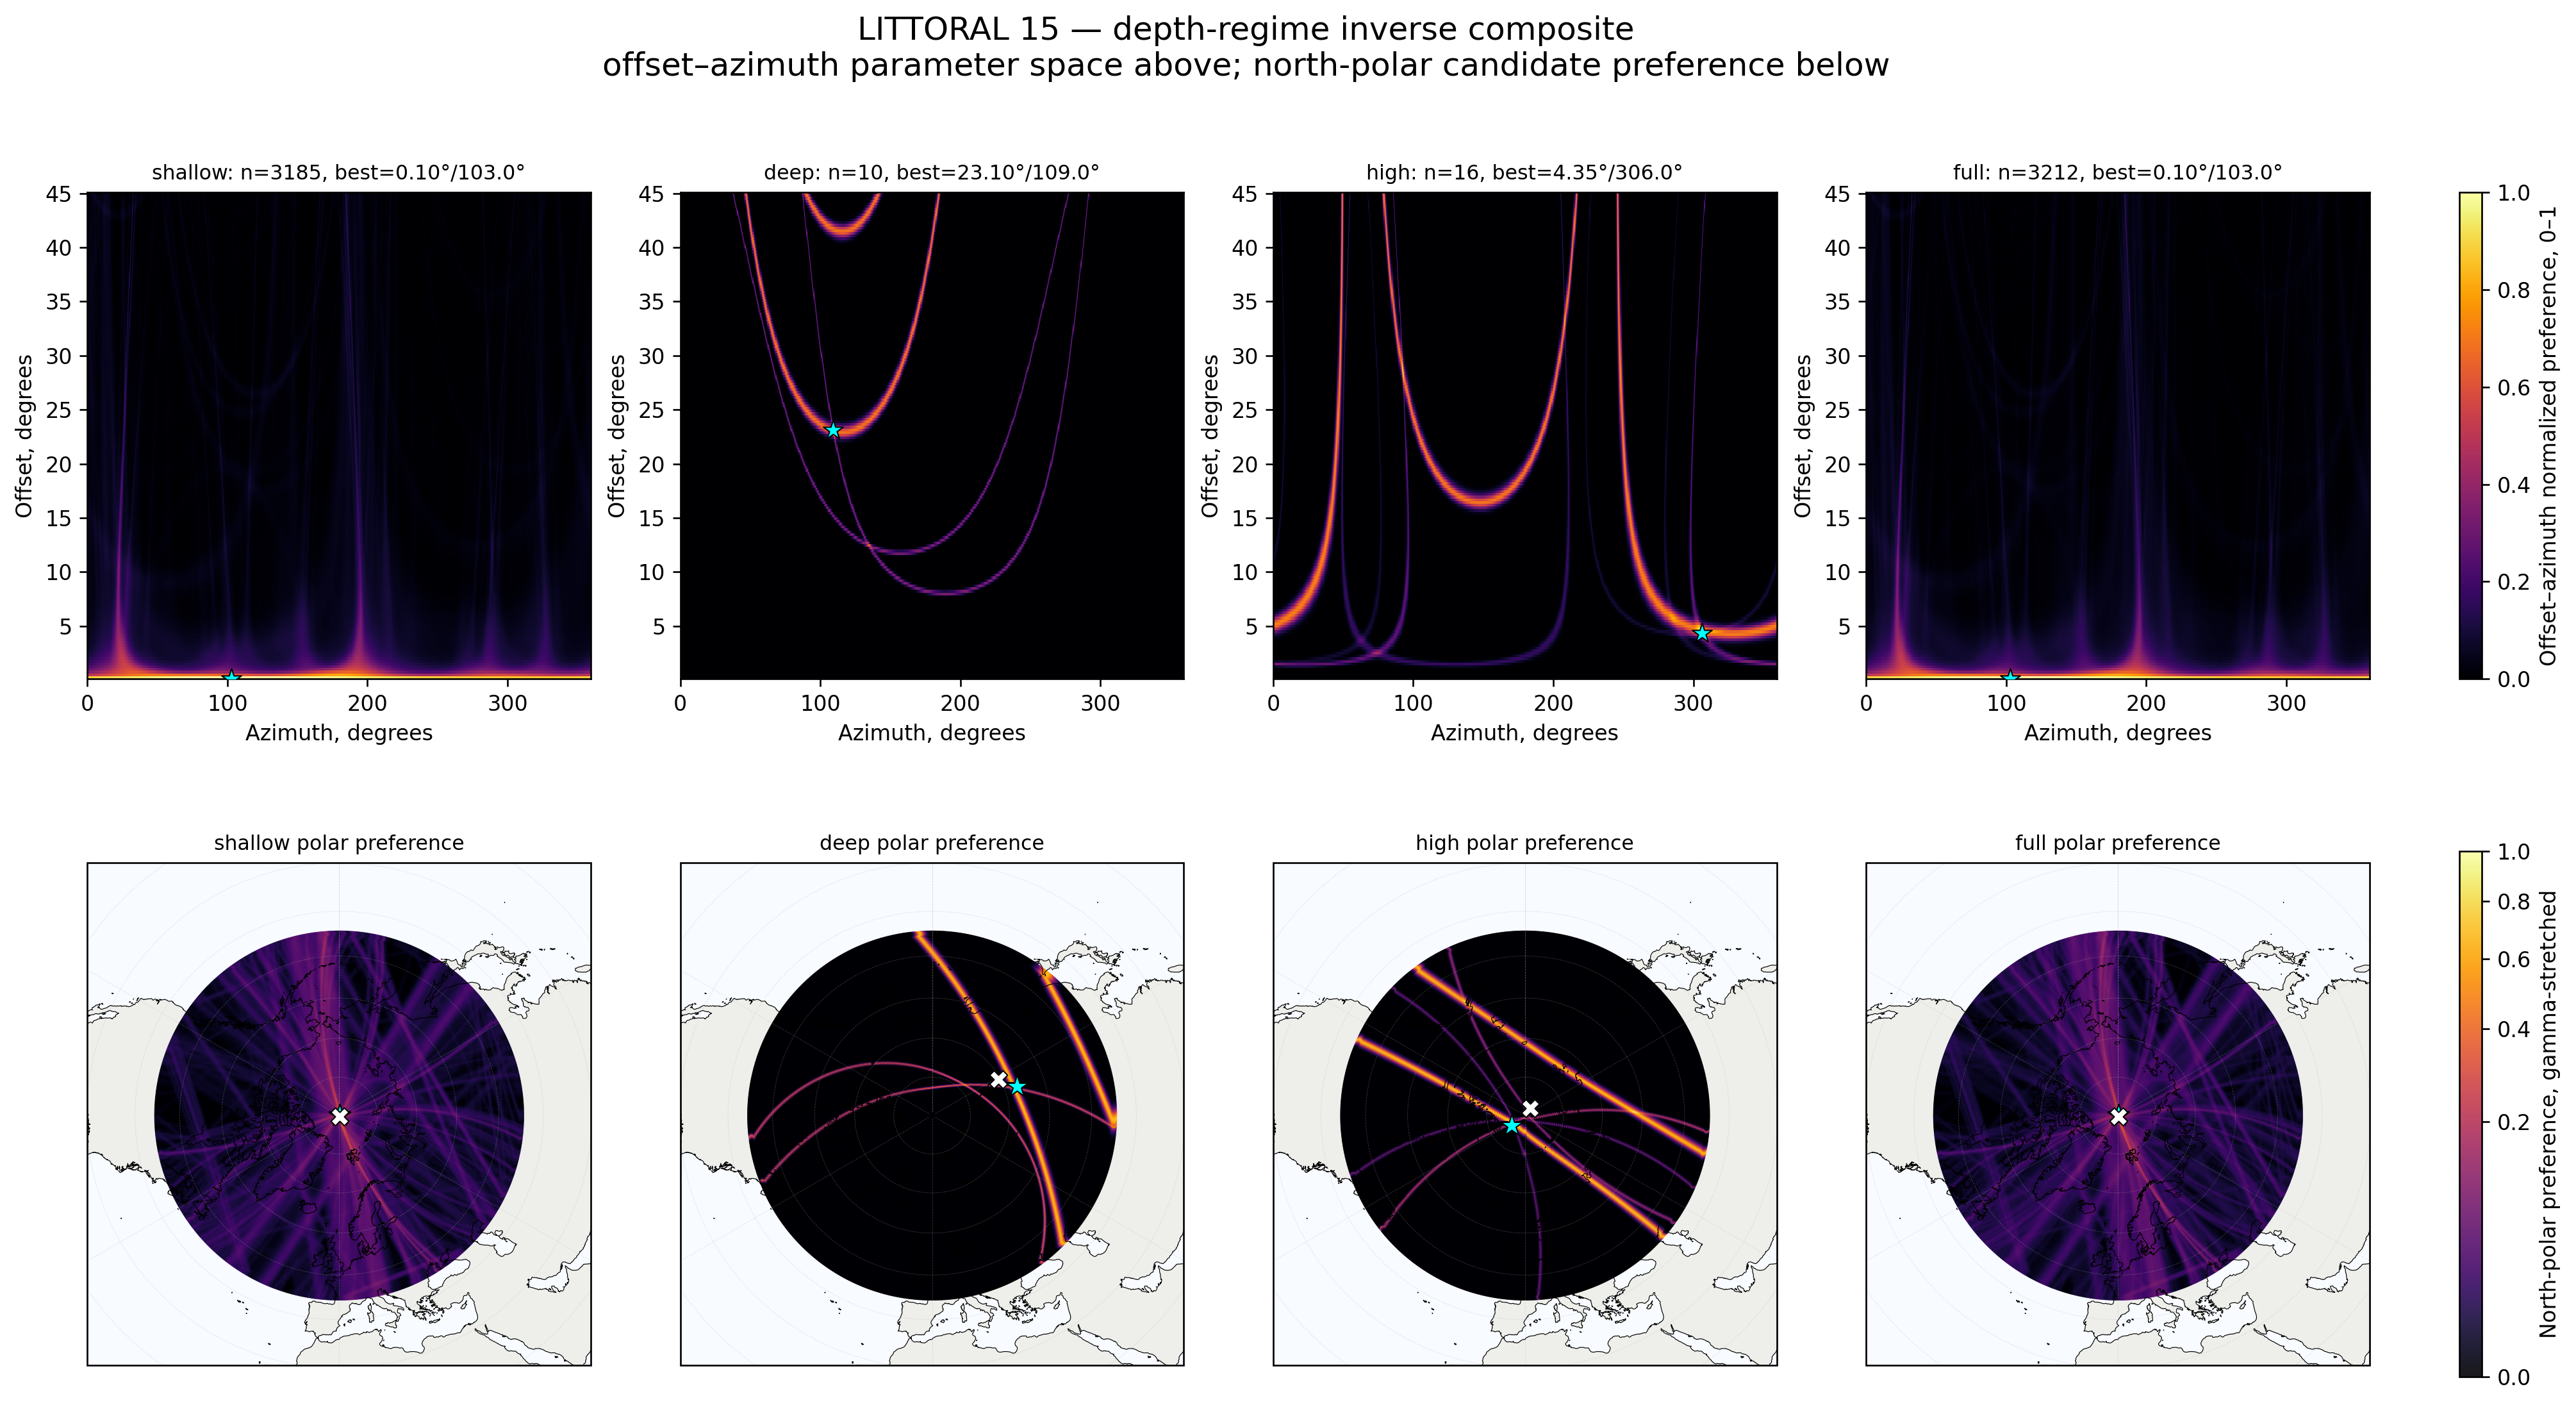
\includegraphics[width=\textwidth]{../outputs/geospatial_15/15_depth_regime_composite.png}
\caption{Depth-regime geodetic inverse composite for reported LITTORAL elevations. The upper row shows normalized preference in offset--azimuth parameter space for shallow, deep, raised, and full reported-elevation cohorts. The lower row maps the corresponding candidate-pole preference in north-polar projection. The shallow and full populations are dominated by near-present, low-offset solutions, while the sparse deep and raised regimes occupy distinct finite-offset solution families. This separation indicates that the reported dataset is not well represented as a single homogeneous geodetic population.}
\label{fig:depth_regime_inverse}
\end{figure*}

The resulting regime separation is the important result. The shallow population is dominated by near-zero polar offsets, consistent with low-amplitude relative sea-level indicators close to the present hydrospheric configuration. By contrast, the sparse deep and raised regimes preferentially illuminate finite-offset structures in the inverse space. In the present run, the deep cohort contains only ten records, so its solution should be treated cautiously; nevertheless, its preferred family is not identical to the shallow solution. The raised cohort likewise occupies a distinct finite-offset family.

This behavior suggests that the merged reported-elevation dataset is better treated as a mixture of geometric regimes than as a single scalar sea-level population. The Beebe example provides the intuitive end-member: an extreme-depth littoral claim cannot be evaluated by asking only whether it lies above or below present sea level. It must be evaluated by asking what global geodetic configuration would make such a shoreline elevation geometrically admissible, and whether other observations independently support the same configuration.

\section{Constraint Over Explanation}

It is important to emphasize that the present analysis does not assume a specific causal mechanism. Instead, it identifies a geometric constraint: the global distribution of RSL indicators is incompatible with isotropic randomness and exhibits structured alignment with an independent anisotropy field.

This constraint narrows the space of viable explanations. Any successful model of global sea-level change must account for:

\begin{itemize}
\item The existence of coherent gradient pathways
\item Their alignment with a global anisotropy field
\item The reduction in integrated pathway resistance relative to random expectation
\end{itemize}

In this sense, the analysis functions as a diagnostic rather than a prescription.

\section{Transition to Broader Implications}

The emergence of coherent global structure in the LITTORAL dataset invites reconsideration of how relative sea-level indicators are interpreted.

Rather than treating each observation as an independent local datum, the dataset may be more fruitfully understood as a distributed measurement of a global geometric transformation.

The final section explores the implications of this perspective and outlines directions for further work.

\section{Discussion}

The central result of this study is the identification of coherent, non-random geometric structure within a global compilation of relative sea-level indicators. This structure is expressed through:

\begin{itemize}
\item Anisotropic gradient pathways in the LITTORAL elevation field
\item Systematic alignment with low-penalty corridors of an independent Mach field
\item Reduced integrated pathway resistance relative to random expectation
\end{itemize}

Taken together, these observations indicate that the dataset encodes a large-scale geometric constraint.

The geodetic inverse analysis strengthens this interpretation by showing that different elevation regimes project into different regions of polar-orientation space. The shallow reported cohort is dominated by near-present geometry, whereas the sparse deep and raised cohorts illuminate finite-offset solution families. This does not by itself establish a rotational event, but it shows that the dataset behaves like a mixture of geometric regimes rather than a single homogeneous sea-level surface.

\subsection{Geometric Interpretation}

The alignment between LITTORAL gradients and the Mach field suggests that the observed RSL indicators are not merely local responses to isolated processes, but components of a global redistribution pattern.

In a rotational framework, such redistribution arises naturally. Changes in the Earth's rotation alter the equilibrium configuration of the geoid, requiring the ocean mass to adjust accordingly. The resulting field is inherently anisotropic, reflecting the geometry of the underlying transformation.

This interpretation is directly anticipated by \citet{fairbridge1961}, who emphasized that sea-level change should be understood as a geodetic phenomenon involving deformation of the Earth's equipotential surface.

\subsection{Relation to Rotational Reorganization Hypotheses}

While the present analysis does not assume a specific mechanism, the observed structure is compatible with frameworks involving large-scale redistribution of mass under changing rotational conditions.

In particular, hypotheses involving partial decoupling between the Earth's core and mantle, or transient reorientation of the rotational axis, would naturally produce:

\begin{itemize}
\item Redistribution of the oceanic bulge
\item Spatially structured relative sea-level change
\item Preferential pathways of adjustment governed by global geometry
\end{itemize}

The LITTORAL dataset provides an empirical basis against which such hypotheses may be tested.

\subsection{Integration with Classical and Modern Frameworks}

It is important to situate these findings within the broader context of sea-level research. Established processes---including glacio-isostatic adjustment, tectonics, sediment compaction, and dynamic oceanography---remain essential components of any comprehensive explanation.

However, these processes are typically treated as locally or regionally dominant. The emergence of a coherent global structure suggests that an additional organizing principle may be present.

The geometric constraint identified here does not replace existing models, but rather imposes boundary conditions on them.

\section{Limitations}

Several limitations must be acknowledged.

\subsection{Sampling Bias}

The LITTORAL dataset is compiled from published literature and therefore reflects uneven geographic and research coverage. Regions with intensive study (e.g., Europe, North America) are overrepresented relative to less-studied areas.

\subsection{Indicator Heterogeneity}

The dataset includes a wide range of indicator types, each with its own formation processes and uncertainties. While this diversity increases coverage, it also introduces variability that may obscure finer-scale structure.

\subsection{Elevation Uncertainty}

Elevation and depth estimates are subject to uncertainties arising from measurement error, datum differences, and post-depositional processes. DEM-based normalization mitigates some of these issues but does not eliminate them.

\subsection{Temporal Aggregation}

The present analysis treats the dataset as temporally aggregated. In reality, the observations span multiple time periods, and their superposition may blur time-dependent structure.

\subsection{Sparse Extreme-Depth Regimes}

The deep inverse regime presently contains only a small number of reported records. Its finite-offset solution family should therefore be interpreted as a diagnostic target rather than a final result. Additional extreme-depth and raised littoral indicators are required before the inferred regime structure can be considered robust. The value of the present analysis is that it defines the test: if such records are real and geometrically coherent, they should converge toward repeatable regions of pole-space under the inverse model.

\section{Future Work}

The results presented here open several avenues for further investigation.

\subsection{Temporal Stratification}

Separating the dataset into time slices would allow the evolution of the geometric structure to be examined. This could reveal whether the observed alignment strengthens or weakens during specific intervals.

\subsection{Depth-Regime Expansion}

Future LITTORAL development should explicitly expand the deep and raised reported-elevation cohorts. Records analogous to the Beebe (1931) Bermuda submerged-beach report should be geocoded, elevation-normalized, and tested as a separate inverse population rather than being averaged into the dense shallow shoreline dataset. This will determine whether extreme-depth littoral indicators form a coherent finite-offset geodetic regime or dissolve under broader sampling.

\subsection{Regional Analysis}

Focused studies of regions such as Dogger Bank may provide higher-resolution insights into gradient structure and its relation to local bathymetry.

\subsection{Integration with Additional Datasets}

Expanding the dataset to include additional sources (e.g., marine sediment cores, seismic stratigraphy) would improve coverage and robustness.

\subsection{Coupling to Dynamical Models}

The geometric constraints identified here can be used to inform and test dynamical models of sea-level change, including those involving rotational or mass redistribution processes.

\subsection{Higher-Order Geometry}

Beyond first-order gradients, higher-order derivatives and curvature measures may reveal additional structure in the dataset.

\section{Conclusion}

We have presented a global, geometry-first analysis of relative sea-level indicators using the LITTORAL dataset. The results demonstrate that:

\begin{itemize}
\item The global distribution of RSL indicators exhibits coherent anisotropic structure
\item This structure aligns with an independently derived Mach field
\item Pathways derived from the data minimize integrated geometric resistance relative to random expectation
\end{itemize}

These findings support the view that relative sea-level change is, at least in part, a manifestation of global geometric processes, as originally emphasized by \citet{fairbridge1961}.

The LITTORAL framework provides a reproducible basis for further exploration of these processes and their implications for Earth's dynamic history.

\section*{Acknowledgments}

The author acknowledges the developers and contributors to the WALIS database and the broader scientific community whose work underpins the LITTORAL dataset.

\section*{Data Availability}

All data, code, and figures used in this study are available at:
\url{https://github.com/nobulart/littoral}

\begin{thebibliography}{}

\bibitem[Fairbridge(1961)]{fairbridge1961}
Fairbridge, R. W. (1961).
\newblock Eustatic Changes in Sea Level.
\newblock In \emph{Physics and Chemistry of the Earth}, Vol. 4, pp. 99--185.
\newblock Pergamon Press.
\newblock \textbf{Seminal work emphasizing geodetic and rotational contributions to sea-level change.}

\bibitem[Beebe(1931)]{beebe1931}
Beebe, W. (1931).
\newblock A submerged beach off Bermuda.
\newblock \emph{Science}, 74(1929), 629--630.
\newblock \url{https://www.science.org/doi/10.1126/science.74.1929.629}
\newblock \textbf{Reports water-worn pebbles, coral fragments, and shallow-water shells from approximately 1,450--1,550 fathoms south-southeast of Bermuda, interpreted by the author as evidence of an in situ submerged sea-beach.}

\bibitem[WALIS Consortium(2020)]{walis2020}
WALIS Consortium (2020).
\newblock The World Atlas of Last Interglacial Shorelines (WALIS).
\newblock \url{https://warmcoasts.eu/world-atlas.html}
\newblock LITTORAL accepted candidate points: 3038.

% Automatically added from outputs/per_source CSVs with >=3 accepted candidate points.
\bibitem[Aharon and Chappell(1986)]{aharon1986}
Aharon and Chappell (1986).
\newblock Oxygen isotopes, sea level changes and the temperature history of a coral reef environment in New Guinea over the last 10\textsuperscript{5} years.
\newblock \url{https://doi.org/10.1016/0031-0182(86)90101-X}
\newblock LITTORAL accepted candidate points: 3.

\bibitem[Allen et al.(1990)]{allen1990}
Allen et al. (1990).
\newblock The Severn Estuary in southwest Britain: its retreat under marine transgression, and fine-sediment regime.
\newblock \url{https://doi.org/10.1016/0037-0738(90)90003-C}
\newblock LITTORAL accepted candidate points: 3.

\bibitem[Aloisi et al.(1978)]{aloisi2011}
Aloisi et al. (1978).
\newblock The Holocene transgression in the Golfe du Lion, southwestern France: Paleogeographic and paleobotanical evolution.
\newblock \url{https://doi.org/10.7202/1000346ar}
\newblock LITTORAL accepted candidate points: 9.

\bibitem[Ballard et al.(2000)]{ballard2000}
Ballard et al. (2000).
\newblock Further evidence of abrupt Holocene drowning of the Black Sea shelf.
\newblock \url{https://doi.org/10.1016/S0025-3227(00)00108-0}
\newblock LITTORAL accepted candidate points: 3.

\bibitem[Barbosa et al.(2018)]{barbosa2018}
Barbosa et al. (2018).
\newblock Late Quaternary infilling of the Assu River embayment and related sea level changes in NE Brazil.
\newblock \url{https://doi.org/10.1016/j.margeo.2018.07.014}
\newblock LITTORAL accepted candidate points: 16.

\bibitem[Barghoorn(1953)]{barghoorn1953}
Barghoorn (1953).
\newblock Recent Changes in Sea Level Along the New England Coast: New Archaeological Evidence.
\newblock LITTORAL accepted candidate points: 3.

\bibitem[Bateman et al.(2011)]{bateman2011}
Bateman et al. (2011).
\newblock The evolution of coastal barrier systems: a case study of the Middle-Late Pleistocene Wilderness barriers, South Africa.
\newblock \url{https://doi.org/10.1016/j.quascirev.2010.10.003}
\newblock LITTORAL accepted candidate points: 4.

\bibitem[Beaman et al.(2008)]{beaman2008}
Beaman et al. (2008).
\newblock New evidence for drowned shelf edge reefs in the Great Barrier Reef, Australia.
\newblock \url{https://doi.org/10.1016/j.margeo.2007.08.001}
\newblock LITTORAL accepted candidate points: 7.

\bibitem[Bilbao-Lasa et al.(2020)]{bilbao-lasa2020}
Bilbao-Lasa et al. (2020).
\newblock Submerged Marine Terraces Identification and an Approach for Numerical Modeling the Sequence Formation in the Bay of Biscay (Northeastern Iberian Peninsula).
\newblock \url{https://doi.org/10.3389/feart.2020.00047}
\newblock LITTORAL accepted candidate points: 17.

\bibitem[Björck et al.(1995)]{bjorck1995}
Björck et al. (1995).
\newblock A REVIEW OF THE HISTORY OF THE BALTIC SEA, 13.0-8.0 ka BP.
\newblock \url{https://doi.org/10.1016/1040-6182(94)00057-C}
\newblock LITTORAL accepted candidate points: 5.

\bibitem[Brooke et al.(2017)]{brooke2017}
Brooke et al. (2017).
\newblock Palaeoshorelines on the Australian continental shelf: Morphology, sea-level relationship and applications to environmental management and archaeology.
\newblock \url{https://doi.org/10.1016/j.csr.2016.12.012}
\newblock LITTORAL accepted candidate points: 32.

\bibitem[Brunovic et al.(2020)]{brunovic2020}
Brunovic et al. (2020).
\newblock Late Pleistocene and Holocene paleoenvironmental reconstruction of a drowned karst isolation basin (Lošinj Channel, NE Adriatic Sea).
\newblock \url{https://doi.org/10.1016/j.palaeo.2020.109587}
\newblock LITTORAL accepted candidate points: 16.

\bibitem[Camoin et al.(2012)]{camoin2012}
Camoin et al. (2012).
\newblock Reef response to sea-level and environmental changes during the last deglaciation: Integrated Ocean Drilling Program Expedition 310, Tahiti Sea Level.
\newblock \url{https://doi.org/10.1130/G32057.1}
\newblock LITTORAL accepted candidate points: 5.

\bibitem[Castillo et al.(2018)]{castillo2018}
Castillo et al. (2018).
\newblock Late Quaternary subsidence of Santa Catalina Island, California Continental Borderland, demonstrated by seismic-reflection data and fossil assemblages from submerged marine terraces.
\newblock \url{https://doi.org/10.1130/B31738.1}
\newblock LITTORAL accepted candidate points: 21.

\bibitem[Cawthra et al.(2015)]{cawthra2015}
Cawthra et al. (2015).
\newblock Submerged shorelines and landscape features offshore of Mossel Bay, South Africa.
\newblock \url{https://doi.org/10.1144/SP411.11}
\newblock LITTORAL accepted candidate points: 7.

\bibitem[Cawthra et al.(2020)]{cawthra2020}
Cawthra et al. (2020).
\newblock Seismic stratigraphy of the inner to mid Agulhas bank, South Africa.
\newblock \url{https://doi.org/10.1016/j.quascirev.2019.105979}
\newblock LITTORAL accepted candidate points: 3.

\bibitem[Cerrone et al.(2021)]{cerrone2021}
Cerrone et al. (2021).
\newblock Development and deformation of marine terraces: Constraints to the evolution of the Campania Plain Quaternary coastal basin (Italy).
\newblock \url{https://doi.org/10.1016/j.geomorph.2021.107725}
\newblock LITTORAL accepted candidate points: 9.

\bibitem[Chappell and Shackleton(1986)]{chappell1986}
Chappell and Shackleton (1986).
\newblock Oxygen isotopes and sea level.
\newblock LITTORAL accepted candidate points: 7.

\bibitem[Chaytor et al.(2008)]{chaytor2008}
Chaytor et al. (2008).
\newblock Measuring vertical tectonic motion at the intersection of the Santa Cruz–Catalina Ridge and Northern Channel Islands platform, California Continental Borderland, using submerged paleoshorelines.
\newblock \url{https://doi.org/10.1130/B26316.1}
\newblock LITTORAL accepted candidate points: 5.

\bibitem[Chen et al.(2017)]{chen2017}
Chen et al. (2017).
\newblock Revisiting the deformed high shoreline of Lake Bonneville.
\newblock \url{https://doi.org/10.1016/j.quascirev.2016.12.019}
\newblock LITTORAL accepted candidate points: 5.

\bibitem[Corliss(1968)]{corliss1968}
Corliss (1968).
\newblock Mysteries Beneath the Sea.
\newblock LITTORAL accepted candidate points: 4.

\bibitem[Cronin et al.(2007)]{cronin2007}
Cronin et al. (2007).
\newblock Rapid sea level rise and ice sheet response to 8,200-year climate event.
\newblock \url{https://doi.org/10.1029/2007GL031318}
\newblock LITTORAL accepted candidate points: 6.

\bibitem[Day(1866)]{day1866}
Day (1866).
\newblock On some remains of a gigantic fossil fish from the Kimmeridge Clay.
\newblock LITTORAL accepted candidate points: 3.

\bibitem[Dickinson et al.(2000)]{dickinson2000}
Dickinson et al. (2000).
\newblock Hydro-Isostatic and Tectonic Influences on Emergent Holocene Paleoshorelines in the Mariana Islands, Western Pacific Ocean.
\newblock LITTORAL accepted candidate points: 3.

\bibitem[Dominguez et al.(1988)]{dominguez1988}
Dominguez et al. (1988).
\newblock Cat Island platform, Bahamas: an incipiently drowned Holocene carbonate shelf.
\newblock LITTORAL accepted candidate points: 5.

\bibitem[Eronen et al.(2001)]{eronen2001}
Eronen et al. (2001).
\newblock Rates of Holocene isostatic uplift and relative sea-level lowering of the Baltic in SW Finland based on studies of isolation contacts.
\newblock LITTORAL accepted candidate points: 4.

\bibitem[Etienne et al.(2021)]{etienne2021}
Etienne et al. (2021).
\newblock Large-scale margin collapses along a partly drowned, isolated carbonate platform (Lansdowne Bank, SW Pacific Ocean).
\newblock \url{https://doi.org/10.1016/j.margeo.2021.106477}
\newblock LITTORAL accepted candidate points: 3.

\bibitem[Fairbridge(1958)]{fairbridge1958}
Fairbridge (1958).
\newblock Dating the latest movements of the Quaternary sea level.
\newblock LITTORAL accepted candidate points: 9.

\bibitem[Fedje et al.(1999)]{fedje1999}
Fedje et al. (1999).
\newblock MODELING PALEOSHORELINES AND LOCATING EARLY HOLOCENE COASTAL SITES IN HAIDA GWAII.
\newblock LITTORAL accepted candidate points: 12.

\bibitem[Ferranti et al.(2017)]{ferranti2017}
Ferranti et al. (2017).
\newblock Uplifted Late Holocene shorelines along the coasts of the Calabrian Arc: geodynamic and seismotectonic implications.
\newblock \url{https://doi.org/10.3301/IJG.2017.13}
\newblock LITTORAL accepted candidate points: 8.

\bibitem[Fleming et al.(1998)]{fleming1998}
Fleming et al. (1998).
\newblock Refining the eustatic sea-level curve since the Last Glacial Maximum using far- and intermediate-field sites.
\newblock LITTORAL accepted candidate points: 12.

\bibitem[Foglini et al.(2015)]{foglini2015}
Foglini et al. (2015).
\newblock Late Quaternary coastal landscape morphology and evolution of the Maltese Islands (Mediterranean Sea) reconstructed from high-resolution seafloor data.
\newblock \url{https://doi.org/10.1144/SP411.12}
\newblock LITTORAL accepted candidate points: 12.

\bibitem[Forbes et al.(2014)]{forbes2014}
Forbes et al. (2014).
\newblock Coastal products of marine transgression in cold-temperate and high-latitude coastal-plain settings: Gulf of St Lawrence and Beaufort Sea.
\newblock \url{https://doi.org/10.1144/SP388.18}
\newblock LITTORAL accepted candidate points: 6.

\bibitem[Garcia et al.(2013)]{garcia2013}
Garcia et al. (2013).
\newblock High resolution seismic study of the Holocene infill of the Elkhorn Slough, central California.
\newblock \url{https://doi.org/10.1016/j.csr.2013.01.012}
\newblock LITTORAL accepted candidate points: 10.

\bibitem[Gayes et al.(1991)]{gayes1991}
Gayes et al. (1991).
\newblock Estuarine Paleoshorelines in Long Island Sound, New York.
\newblock LITTORAL accepted candidate points: 7.

\bibitem[Gharibreza et al.(2016)]{gharibreza2016}
Gharibreza et al. (2016).
\newblock Evolutionary trend of paleoshorelines in the Coastal Makran zone (Southeast Iran) since the mid-Holocene.
\newblock \url{https://doi.org/10.1016/j.quaint.2015.06.030}
\newblock LITTORAL accepted candidate points: 3.

\bibitem[Greenwood(1868)]{greenwood1868}
Greenwood (1868).
\newblock Submerged Forests, and Raised Sea-Beaches.
\newblock LITTORAL accepted candidate points: 4.

\bibitem[Hine et al.(1984)]{hine1984}
Hine et al. (1984).
\newblock CAY SAL BANK, BAHAMAS — A PARTIALLY DROWNED CARBONATE PLATFORM.
\newblock \url{https://doi.org/10.1016/0025-3227(84)90091-4}
\newblock LITTORAL accepted candidate points: 4.

\bibitem[Hoffmann et al.(2009)]{hoffmann2009}
Hoffmann et al. (2009).
\newblock Drowned carbonate platforms in the Bismarck Sea, Papua New Guinea.
\newblock \url{https://doi.org/10.1007/s11001-010-9079-8}
\newblock LITTORAL accepted candidate points: 6.

\bibitem[Hovland et al.(1981)]{hovland1981}
Hovland et al. (1981).
\newblock A SUBMERGED BEACH BETWEEN NORWAY AND EKOFISK IN THE NORTH SEA.
\newblock \url{https://doi.org/10.1016/0025-3227(81)90123-7}
\newblock LITTORAL accepted candidate points: 6.

\bibitem[Jara-Muñoz et al.(2017)]{jaramuniz2017}
Jara-Muñoz et al. (2017).
\newblock Quantifying offshore forearc deformation and splay-fault slip using drowned Pleistocene shorelines, Arauco Bay, Chile.
\newblock \url{https://doi.org/10.1002/2016JB013339}
\newblock LITTORAL accepted candidate points: 5.

\bibitem[Jelgersma et al.(2002)]{jelgersma2002}
Jelgersma et al. (2002).
\newblock Relative sea level changes and some effects on muddy coasts.
\newblock \url{https://doi.org/10.1016/S1568-2692(02)80079-1}
\newblock LITTORAL accepted candidate points: 3.

\bibitem[Karig et al.(1970)]{karig1970}
Karig et al. (1970).
\newblock Sediment-capped guyots in the Mid-Pacific Mountains\*.
\newblock \url{https://doi.org/10.1016/0011-7471(70)90029-X}
\newblock LITTORAL accepted candidate points: 5.

\bibitem[Keigwin et al.(2006)]{keigwin2006}
Keigwin et al. (2006).
\newblock Rapid sea-level rise and Holocene climate in the Chukchi Sea.
\newblock \url{https://doi.org/10.1130/G22712.1}
\newblock LITTORAL accepted candidate points: 4.

\bibitem[Koba et al.(1982)]{koba1982}
Koba et al. (1982).
\newblock Late Holocene eustatic sea-level changes deduced from geomorphological features and their radiocarbon dates in the Ryukyu Islands, Japan.
\newblock \url{https://doi.org/10.1016/0031-0182(82)90024-4}
\newblock LITTORAL accepted candidate points: 4.

\bibitem[Lambeck et al.(1996)]{lambeck1996b}
Lambeck et al. (1996).
\newblock Shoreline reconstructions for the Persian Gulf since the last glacial maximum.
\newblock LITTORAL accepted candidate points: 12.

\bibitem[Lebrec et al.(2022)]{lebrec2022}
Lebrec et al. (2022).
\newblock Morphology and distribution of submerged palaeoshorelines: Insights from the North West Shelf of Australia.
\newblock \url{https://doi.org/10.1016/j.earscirev.2021.103864}
\newblock LITTORAL accepted candidate points: 14.

\bibitem[Lee et al.(2009)]{lee2009}
Lee et al. (2009).
\newblock OSL dating of paleoshorelines at Lagkor Tso, western Tibet.
\newblock \url{https://doi.org/10.1016/j.quageo.2009.02.003}
\newblock LITTORAL accepted candidate points: 5.

\bibitem[Letham et al.(2018)]{letham2018}
Letham et al. (2018).
\newblock Archaeological Survey of Dynamic Coastal Landscapes and Paleoshorelines: Locating Early Holocene Sites in the Prince Rupert Harbour Area, British Columbia, Canada.
\newblock \url{https://doi.org/10.1080/00934690.2018.1441575}
\newblock LITTORAL accepted candidate points: 4.

\bibitem[Lidz et al.(1991)]{lidz1991}
Lidz et al. (1991).
\newblock Paleoshorelines, Reefs, and a Rising Sea: South Florida, U.S.A..
\newblock LITTORAL accepted candidate points: 5.

\bibitem[Liu et al.(2018)]{liu2018}
Liu et al. (2018).
\newblock Early to Middle Holocene sea level fluctuation, coastal progradation and the Neolithic occupation in the Yaojiang Valley of southern Hangzhou Bay, Eastern China.
\newblock \url{https://doi.org/10.1016/j.quascirev.2018.04.010}
\newblock LITTORAL accepted candidate points: 5.

\bibitem[Maio et al.(2014)]{maio2014}
Maio et al. (2014).
\newblock Late Holocene marine transgression and the drowning of a coastal forest: Lessons from the past, Cape Cod, Massachusetts, USA.
\newblock \url{https://doi.org/10.1016/j.palaeo.2013.11.018}
\newblock LITTORAL accepted candidate points: 6.

\bibitem[Mancini et al.(2007)]{mancini2007}
Mancini et al. (2007).
\newblock Geomorphological, paleontological and 87Sr/86Sr isotope analyses of early Pleistocene paleoshorelines to define the uplift of Central Apennines (Italy).
\newblock \url{https://doi.org/10.1016/j.yqres.2007.01.005}
\newblock LITTORAL accepted candidate points: 5.

\bibitem[Martínez-Martos et al.(2016)]{martinez-martos2016}
Martínez-Martos et al. (2016).
\newblock Buried marine-cut terraces and submerged marine-built terraces: The Carchuna-Calahonda coastal area (southeast Iberian Peninsula).
\newblock \url{https://doi.org/10.1016/j.geomorph.2016.04.010}
\newblock LITTORAL accepted candidate points: 6.

\bibitem[Matthews et al.(1967)]{matthews1967}
Matthews et al. (1967).
\newblock LATE QUATERNARY MARINE FOSSILS FROM FROBISHER BAY (BAFFIN ISLAND, N.W.T., CANADA).
\newblock \url{https://doi.org/10.1016/0031-0182(67)90018-1}
\newblock LITTORAL accepted candidate points: 19.

\bibitem[Mitchell(2005)]{mitchell2005}
Mitchell (2005).
\newblock When the Sea Flooded Britain: A Catastrophic Late Holocene Isostatic Interlude along the Eastern Seaboard of England and Scotland.
\newblock LITTORAL accepted candidate points: 9.

\bibitem[Moller et al.(2000)]{moller20000}
Moller et al. (2000).
\newblock Submerged littoral sediments, beach ridges and wavecut platforms off Troms, North Norway: revisiting old questions.
\newblock LITTORAL accepted candidate points: 6.

\bibitem[Mouslopoulou et al.(2015)]{mouslopoulou2015}
Mouslopoulou et al. (2015).
\newblock Formation of Late Quaternary paleoshorelines in Crete, Eastern Mediterranean.
\newblock \url{https://doi.org/10.1016/j.epsl.2015.09.007}
\newblock LITTORAL accepted candidate points: 14.

\bibitem[Ott et al.(2019)]{ott2019}
Ott et al. (2019).
\newblock Pleistocene terrace formation, Quaternary rock uplift rates and geodynamics of the Hellenic Subduction Zone revealed from dating of paleoshorelines on Crete, Greece.
\newblock \url{https://doi.org/10.1016/j.epsl.2019.115757}
\newblock LITTORAL accepted candidate points: 7.

\bibitem[Peterson et al.(2010)]{peterson2010}
Peterson et al. (2010).
\newblock Composition, age, and depositional rates of shoreface deposits under barriers and beach plains of the Columbia River littoral cell, USA.
\newblock \url{https://doi.org/10.1016/j.margeo.2010.02.004}
\newblock LITTORAL accepted candidate points: 9.

\bibitem[Peterson et al.(2016)]{peterson2016}
Peterson et al. (2016).
\newblock Accommodation space controls on incised-valley sediment accumulation rates during the Holocene marine transgression (0–11 ka) in Grays Harbor, a large meso-tidal estuary, Washington, USA.
\newblock \url{https://doi.org/10.1016/j.margeo.2016.06.012}
\newblock LITTORAL accepted candidate points: 11.

\bibitem[Pretorius et al.(2016)]{pretorius2016}
Pretorius et al. (2016).
\newblock Submerged shoreline preservation and ravinement during rapid postglacial sea-level rise and subsequent “slowstand”.
\newblock \url{https://doi.org/10.1130/B31381.1}
\newblock LITTORAL accepted candidate points: 5.

\bibitem[Rao et al.(1989)]{rao1989}
Rao et al. (1989).
\newblock Holocene marine transgression as interpreted from bathymetry and sand grain size parameters off Gopalpur.
\newblock LITTORAL accepted candidate points: 4.

\bibitem[Rokoengen et al.(1982)]{rokoengen1982}
Rokoengen et al. (1982).
\newblock Description and dating of a submerged beach in the northern North Sea.
\newblock \url{https://doi.org/10.1016/0025-3227(82)90056-1}
\newblock LITTORAL accepted candidate points: 12.

\bibitem[Sager et al.(1992)]{sager1992}
Sager et al. (1992).
\newblock Mississippi–Alabama Outer Continental Shelf Topographic Features Formed during the Late Pleistocene–Holocene Transgression.
\newblock LITTORAL accepted candidate points: 7.

\bibitem[Schimanski et al.(2005)]{schimanski2005}
Schimanski et al. (2005).
\newblock Deglacial and Holocene evolution of the Vietnam shelf: stratigraphy, sediments and sea-level change.
\newblock \url{https://doi.org/10.1016/j.margeo.2004.11.001}
\newblock LITTORAL accepted candidate points: 3.

\bibitem[Simonarson et al.(2002)]{simonarson2002}
Simonarson et al. (2002).
\newblock Late-Holocene sea-level changes in south and southwest Iceland reconstructed from littoral molluscan stratigraphy.
\newblock \url{https://doi.org/10.1191/0959683602hl530rp}
\newblock LITTORAL accepted candidate points: 3.

\bibitem[Smith et al.(2011)]{smith2011}
Smith et al. (2011).
\newblock The early Holocene sea level rise.
\newblock \url{https://doi.org/10.1016/j.quascirev.2011.04.019}
\newblock LITTORAL accepted candidate points: 5.

\bibitem[Sørensen et al.(2010)]{soerensen2010}
Sørensen et al. (2010).
\newblock Late Pleistocene and Holocene whale remains (Cetacea) from Denmark and adjacent countries: Species, distribution, chronology, and trace element concentrations.
\newblock \url{https://doi.org/10.1111/j.1748-7692.2009.00356.x}
\newblock LITTORAL accepted candidate points: 51.

\bibitem[Sonnenburg et al.(2012)]{sonnenburg2012}
Sonnenburg et al. (2012).
\newblock Holocene paleoshorelines, water levels and submerged prehistoric site potential of Rice Lake (Ontario, Canada).
\newblock \url{https://doi.org/10.1016/j.jas.2012.05.035}
\newblock LITTORAL accepted candidate points: 7.

\bibitem[Spampinato et al.(2012)]{spampinato2012}
Spampinato et al. (2012).
\newblock Raised Holocene paleo-shorelines along the Capo Schisò coast, Taormina: New evidence of recent co-seismic deformation in northeastern Sicily (Italy).
\newblock \url{https://doi.org/10.1016/j.jog.2011.11.007}
\newblock LITTORAL accepted candidate points: 15.

\bibitem[Sprigg et al.(1979)]{sprigg1979}
Sprigg et al. (1979).
\newblock STRANDED AND SUBMERGED SEA-BEACH SYSTEMS OF SOUTHEAST SOUTH AUSTRALIA AND THE AEOLIAN DESERT CYCLE.
\newblock \url{https://doi.org/10.1016/0037-0738(79)90022-8}
\newblock LITTORAL accepted candidate points: 28.

\bibitem[Taira(1975)]{taira1975}
Taira (1975).
\newblock Holocene crustal movements in Taiwan as indicated by radiocarbon dating of marine fossils and driftwood.
\newblock \url{https://doi.org/10.1016/0040-1951(75)90057-8}
\newblock LITTORAL accepted candidate points: 29.

\bibitem[Thomas et al.(2009)]{thomas2009}
Thomas et al. (2009).
\newblock Penultimate Deglacial Sea-Level Timing from Uranium/Thorium Dating of Tahitian Corals.
\newblock \url{https://doi.org/10.1126/science.1168754}
\newblock LITTORAL accepted candidate points: 6.

\bibitem[Vogt and Conolly(1971)]{vogt1971}
Vogt and Conolly (1971).
\newblock Tasmantid Guyots, the Age of the Tasman Basin, and Motion between the Australia Plate and the Mantle.
\newblock \url{https://doi.org/10.1130/0016-7606(1971)82}
\newblock LITTORAL accepted candidate points: 10.

\bibitem[Vogt et al.(1984)]{vogt1984}
Vogt et al. (1984).
\newblock The Geisha Guyots: Multibeam Bathymetry and Morphometric Interpretation.
\newblock \url{https://doi.org/10.1029/JB089iB13p11085}
\newblock LITTORAL accepted candidate points: 13.

\bibitem[Wang et al.(2015)]{wang2015}
Wang et al. (2015).
\newblock The record of mid-Holocene maximum landward marine transgression in the west coast of Bohai Bay, China.
\newblock \url{https://doi.org/10.1016/j.margeo.2014.11.013}
\newblock LITTORAL accepted candidate points: 6.

\bibitem[Webster et al.(2004)]{webster2004}
Webster et al. (2004).
\newblock Coralgal composition of drowned carbonate platforms in the Huon Gulf, Papua New Guinea; implications for lowstand reef development and drowning.
\newblock \url{https://doi.org/10.1016/S0025-3227(03)00356-6}
\newblock LITTORAL accepted candidate points: 3.

\bibitem[Woodroffe(1981)]{woodroffe1981}
Woodroffe (1981).
\newblock Mangrove swamp stratigraphy and Holocene transgression, Grand Cayman Island, West Indies.
\newblock \url{https://doi.org/10.1016/0025-3227(81)90085-2}
\newblock LITTORAL accepted candidate points: 21.

\bibitem[Yanchilina et al.(2017)]{yanchilina2017}
Yanchilina et al. (2017).
\newblock Compilation of geophysical, geochronological, and geochemical evidence indicates a rapid Mediterranean-derived submergence of the Black Sea's shelf and subsequent substantial salinification in the early Holocene.
\newblock \url{https://doi.org/10.1016/j.margeo.2016.11.001}
\newblock LITTORAL accepted candidate points: 3.

\bibitem[Yanko-Hombach et al.(2014)]{yanko-hombach2014}
Yanko-Hombach et al. (2014).
\newblock Holocene marine transgression in the Black Sea: New evidence from the northwestern Black Sea shelf.
\newblock \url{https://doi.org/10.1016/j.quaint.2013.07.027}
\newblock LITTORAL accepted candidate points: 24.

\bibitem[Zanchetta et al.(2011)]{zanchetta2011}
Zanchetta et al. (2011).
\newblock New insights on the Holocene marine transgression in the Bahía Camarones (Chubut, Argentina).
\newblock \url{https://doi.org/10.3301/IJG.2011.20}
\newblock LITTORAL accepted candidate points: 11.

\bibitem[Zhou et al.(2014)]{zhou2014}
Zhou et al. (2014).
\newblock Fluvial system development and subsequent marine transgression in Yellow River (Huanghe) delta and its adjacent sea regions during last glacial maximum to early Holocene.
\newblock \url{https://doi.org/10.1016/j.csr.2014.06.012}
\newblock LITTORAL accepted candidate points: 12.

\bibitem[Stone(2026)]{stone2026_euler_mach}
Stone, C. (2026).
\newblock Geometric Structure of Euler Pole Compatibility Space: A Constraint-Based Analysis of Rotational Admissibility.
\newblock \url{https://www.academia.edu/165291904/Geometric_Structure_of_Euler_Pole_Compatibility_Space_A_Constraint_Based_Analysis_of_Rotational_Admissibility}
\newblock \textbf{Introduces the Mach compatibility field and demonstrates that admissible Euler poles are constrained by global topographic anisotropy, forming ridge–corridor structures central to the LITTORAL framework.}

\bibitem[Hovland and Rokoengen(1994)]{hovland1994}
Hovland, M., \& Rokoengen, K. (1994).
\newblock Pockmarks in the Norwegian Sea and their potential significance for gas hydrate formation.
\newblock \emph{Marine Geology}, 119(1–2), 49–73.

\bibitem[Mitrovica and Milne(2003)]{mitrovica2003}
Mitrovica, J. X., \& Milne, G. A. (2003).
\newblock On post-glacial sea level: I. General theory.
\newblock \emph{Geophysical Journal International}, 154(2), 253–267.

\bibitem[Lambeck et al.(2014)]{lambeck2014}
Lambeck, K., Rouby, H., Purcell, A., Sun, Y., \& Sambridge, M. (2014).
\newblock Sea level and global ice volumes from the Last Glacial Maximum to the Holocene.
\newblock \emph{Proceedings of the National Academy of Sciences}, 111(43), 15296–15303.

\bibitem[Milne et al.(2005)]{milne2005}
Milne, G. A., Mitrovica, J. X., \& Schrag, D. P. (2005).
\newblock Estimating past continental ice volume from sea-level data.
\newblock \emph{Quaternary Science Reviews}, 24(5–6), 545–560.

\end{thebibliography}

\end{document}
